% ==========================================================================
%  How Many Samples Does a Generative Evaluation Need?
%  Intrinsic Dimension and the Design of Distributional Comparisons
%
%  Typeset with the JMLR style (jmlr2e.sty, preprint option) and the
%  references in references.bib. Build: python tools/build_paper.py.
%  The address of the software repository is set by \repourl below.
%
%  Every measured number is computed from results/ by tools/paper_numbers.py;
%  tests/test_manuscript.py checks the numbers, the citations and the
%  figures against the artifacts. The source is pure ASCII.
% ==========================================================================
\documentclass[twoside,11pt]{article}

\usepackage[T1]{fontenc}
\IfFileExists{lmodern.sty}{\usepackage{lmodern}}{%
  \IfFileExists{courier.sty}{\usepackage{courier}}{}%
  \IfFileExists{helvet.sty}{\usepackage[scaled=0.92]{helvet}}{}}
\usepackage{amsmath}
\usepackage{amssymb}
\usepackage{amsthm}
\IfFileExists{newtxtext.sty}{\usepackage{newtxtext}\usepackage{newtxmath}}%
                            {\usepackage{mathptmx}}
\IfFileExists{helvet.sty}{\usepackage[scaled=0.92]{helvet}}{}

\usepackage[preprint]{jmlr2e}
\usepackage{lastpage}
\raggedbottom

\IfFileExists{newtxtext.sty}{\usepackage{microtype}}%
                            {\usepackage[protrusion=true,expansion=false]{microtype}}
\usepackage{enumitem}
\setlist{itemsep=2pt, topsep=4pt, parsep=0pt, leftmargin=1.8em}
\usepackage{booktabs}
\usepackage{tabularx}
\usepackage{adjustbox}
\emergencystretch=3em
\widowpenalty=10000
\clubpenalty=10000

\hypersetup{colorlinks=true, linkcolor=black, citecolor=black,
            urlcolor=black, breaklinks=true}
\usepackage[nameinlink]{cleveref}

% Theorem environments with separate counters: Propositions 1-4, Lemma 1,
% Definitions 1-7, Assumptions A1-A3.
\theoremstyle{plain}
\newtheorem{prop}{Proposition}
\newtheorem{lem}{Lemma}
\theoremstyle{definition}
\newtheorem{defn}{Definition}
\newtheorem{assumption}{Assumption}
\renewcommand{\theassumption}{A\arabic{assumption}}
\theoremstyle{remark}
\newtheorem{rem}{Remark}
\crefname{prop}{Proposition}{Propositions}
\crefname{lem}{Lemma}{Lemmas}
\crefname{defn}{Definition}{Definitions}
\crefname{rem}{Remark}{Remarks}
\crefname{assumption}{Assumption}{Assumptions}
\crefname{section}{Section}{Sections}
\crefname{appendix}{Appendix}{Appendices}
\crefname{table}{Table}{Tables}
\crefname{figure}{Figure}{Figures}
\crefname{equation}{Equation}{Equations}

% ------------------------------- macros -----------------------------------
\newcommand{\Wtwo}{\ensuremath{W_2}}
\newcommand{\deff}{\ensuremath{d_{\mathrm{eff}}}}
\newcommand{\dhat}{\ensuremath{\hat{d}}}
\newcommand{\Ups}{\ensuremath{\Upsilon}}
\newcommand{\UpsN}{\ensuremath{\Upsilon_{N}}}
\newcommand{\UpsT}{\ensuremath{\tilde{\Upsilon}}}
\newcommand{\UpsTM}{\ensuremath{\tilde{\Upsilon}_{M}}}
\newcommand{\certgen}{\textsf{certgen}}
\DeclareMathOperator{\E}{\mathbb{E}}
\DeclareMathOperator{\Var}{Var}
\DeclareMathOperator{\Cov}{Cov}
\DeclareMathOperator{\sd}{sd}
\DeclareMathOperator*{\argmin}{arg\,min}
\newcommand{\R}{\ensuremath{\mathbb{R}}}
\newcommand{\Prob}{\ensuremath{\mathbb{P}}}
\newcommand{\MDD}{\ensuremath{\mathrm{MDD}}}

% address of the software repository
\newcommand{\repourl}{\url{https://github.com/kahyaoglu20/certgen}}

% ------------------------------- heading ----------------------------------
\jmlrheading{}{2026}{1-\pageref{LastPage}}{}{}{}{\"Omer Kahyao\u{g}lu}
\ShortHeadings{How Many Samples Does a Generative Evaluation Need?}%
              {Kahyao\u{g}lu}
\firstpageno{1}

\begin{document}

\title{How Many Samples Does a Generative Evaluation Need?\\
Intrinsic Dimension and the Design of Distributional Comparisons}

\author{\name \"Omer Kahyao\u{g}lu \email \textnormal{kahyaoglu20@itu.edu.tr} \\
       \hspace*{\fill}{\small\textnormal{math.kahyaoglu@gmail.com}} \\
       \addr Department of Mathematical Engineering\\
       Faculty of Science and Letters\\
       Istanbul Technical University\\
       Istanbul, T\"urkiye}

\maketitle

\begin{abstract}%
Generative models are routinely compared through the distance between a
real and a synthetic sample, yet the sample size needed to resolve a
difference of interest is rarely determined. We develop a framework for
designing and reporting evaluations based on the plug-in 2-Wasserstein
distance. Its central object is the resolution floor, the distance between
two disjoint real samples of equal size, which is strictly positive and
decays at a rate set by the intrinsic dimension of the data. Inverting the
fitted decay gives a prospective sample-size rule. Because the rule is valid
only where a single power law describes the decay, we report the size, power
and severity of the test for that condition. The floor also yields a
floor-corrected skill score, a two-sided test that exposes memorisation, a
minimum detectable difference at stated error rates and an equivalence test.
For latent-generative Wasserstein certificates, the floor determines the
dimension above which no certificate of the standard form can be
informative; we tabulate this limit for up to $32\,768$ samples and replace
the decoder's Lipschitz constant by the transport cost of the latent optimal
coupling, which on trained decoders is within $1.15\times$ of the exact
distance, whereas spectral-norm certificates exceed it by factors of
$12$--$120$. On eight tabular benchmark encodings, the smallest resolvable
difference at $4\,000$ samples per side ranges from $1.4\%$ of the
attainable skill range to $4.5$ times that range, so resolution has to be
determined for each benchmark.
\end{abstract}

\begin{keywords}
generative model evaluation, optimal transport, Wasserstein distance,
intrinsic dimension, power analysis, sample-size planning, tabular data,
reproducibility
\end{keywords}

% ==========================================================================
\section{Introduction}\label{sec:intro}

A generative model is usually evaluated by drawing a synthetic sample,
computing a discrepancy between it and a sample of real data, and comparing
the result with the discrepancies of competing models. The Fr\'echet
Inception Distance \citep{heusel2017} plays this role for images; for
tabular data, practice combines column-wise statistics, pairwise
dependence scores and joint distances such as the Wasserstein distance
\citep{patki2016,yang2024}. In every case the reported number is an estimate
computed from finite samples, and two of its statistical properties are well
documented. Its expectation depends on the sample size in a way that differs
between models \citep{chong2020}, and its sampling variability can be as
large as the differences that are reported between models
\citep{card2020,bouthillier2021}.

These properties raise a design question that precedes any comparison: at a
given sample size, which differences can the evaluation resolve, and how
many samples are needed to resolve a difference of a given size? In
experimental design this question is answered by a power analysis carried
out before data are collected. Existing remedies in generative evaluation
work after the fact, by correcting a score for its bias or attaching error
bars to it; none computes, from the real data alone and before a model is
trained, the sample size required to resolve a target difference.

This paper develops such a design step for evaluations based on the plug-in
2-Wasserstein distance $\Wtwo$. The starting point is an elementary
observation. Two independent samples from the same distribution are at a
strictly positive $\Wtwo$ distance from each other, and the typical size of that distance, which we call the \emph{resolution floor}, decays with the sample size $n$ approximately as $n^{-1/d}$, where $d$ is an intrinsic
dimension of the distribution \citep{weedbach2019}. The floor can be
measured on real data alone by repeatedly splitting a data set into two
disjoint halves. Its level, its rate of decay and its variability then
determine three quantities of practical interest: the sample size at which
the floor falls below a target, the smallest difference between two models
that an evaluation can resolve, and whether a certificate of the standard
latent-generative form can be informative at the available sample size.

A concrete case shows why this step matters. On the numeric columns of the
\texttt{adult} census benchmark with $250$ samples per side, the distance of
a generator that samples every column independently of the others differs
from the floor by $0.017$, while its standard deviation across random seeds
is $0.222$. At this sample size an evaluation cannot distinguish a generator
that removes every dependence between the columns from a generator that
reproduces the data distribution exactly.

A sample-size rule obtained by extrapolating a fitted power law is only as
reliable as the assumption that a single power law describes the decay. We
therefore treat the test of this assumption as a statistical instrument in
its own right, and we measure its size, its power and the severity of its
non-rejections through the same implementation that practitioners use.

\subsection{Contributions}\label{sec:intro-contributions}

\begin{enumerate}[label=(\roman*), itemsep=4pt]
\item \textbf{A design calculus for generative evaluation}
  (\cref{sec:floor,sec:sizing}). We define the resolution floor
  (\cref{def:floor}), show that it is non-degenerate for $\Wtwo$ and
  degenerate for unbiased statistics such as the maximum mean discrepancy
  (\cref{prop:floor}), and invert the fitted floor law into a sample-size
  prescription whose sensitivity to the fitted parameters we derive
  (\cref{prop:inversion}). The prescription is reported as an interval with
  measured coverage, and no prescription is returned when the decay
  exponent is not identified.
\item \textbf{Operating characteristics of the specification test}
  (\cref{sec:sizing-spec,sec:sizing-size,sec:sizing-power,sec:sizing-severity}).
  We show that goodness of fit cannot detect departures from a single power
  law, adopt a parametric-bootstrap \citep{efron1979} curvature test, and report its size as a
  function of the rate regime, its power as a function of the precision of
  the floor measurement, and the severity of each non-rejection.
\item \textbf{Floor-corrected reporting} (\cref{sec:reporting}). We define
  a skill score relative to a hierarchy of reference generators, show that
  a one-sided floor test rewards memorisation and replace it by a two-sided
  test with a null-calibrated leakage screen, and define the minimum
  detectable difference and an equivalence test at stated error rates.
\item \textbf{Limits of latent-generative certificates}
  (\cref{sec:cert,sec:pullback}). We identify the statistical term of a standard
  certificate decomposition as the component that no computation can
  reduce, give a vacuity criterion (\cref{prop:vacuity}), tabulate the
  resulting dimension limit for $N \leq 32\,768$ in the units of a measured
  dimension estimate, test its transfer to non-isotropic, lattice and
  heavy-tailed laws, and replace the Lipschitz step of the certificate by
  an exactly computable coupling cost (\cref{lem:pushforward,prop:ppc}).
\item \textbf{An empirical study} (\cref{sec:empirical}). On eleven
  table--encoding cells from nine public benchmarks we report fitted floor
  laws, the measured scope of the sizing rule, a resolution atlas computed
  without training any model, and certification margins.
\end{enumerate}

The software implementing every procedure, the committed results from which
every number in this paper is computed, and machine-checked proofs of the
formal statements are described in \cref{sec:implementation}.

\subsection{Organisation}\label{sec:intro-organisation}

\Cref{sec:background} reviews related work. \Cref{sec:floor} introduces
the resolution floor and its rate. \Cref{sec:sizing} derives the
sample-size rule and characterises the test that licenses it.
\Cref{sec:reporting} turns the floor into reporting tools and summarises
the resulting procedure in \cref{fig:procedure}.
\Cref{sec:cert,sec:pullback} treat latent-generative certificates.
\Cref{sec:empirical} reports the benchmark study, \cref{sec:implementation}
the implementation, and \cref{sec:discussion} discusses scope and
limitations. Proofs are collected in \cref{app:proofs} and experimental
details in \cref{app:details}.

% ==========================================================================
\section{Related Work}\label{sec:background}

\paragraph{Bias and variability of generative metrics.}
\citet{chong2020} show that the Fr\'echet Inception Distance and the
Inception Score \citep{salimans2016} are biased in finite samples and that the bias depends on
the model, so that one model can appear better than another because its
bias is smaller; they correct for it by extrapolating to infinite sample
size. \citet{jayasumana2024} point out that the Fr\'echet distance assumes Gaussian features, and \citet{chen2026} shows that a statistic built from the first two moments
can be gamed: on ImageNet, images constructed to reproduce nothing but the
mean and covariance of the reference features score a Fr\'echet distance
of $24.7$, better than the $58.6$ of held-out real images. Diagnostic
refinements separate fidelity from coverage
\citep{sajjadi2018,kynkanniemi2019}. \citet{dufour2026} measure the Fr\'echet distance across both training
and sampling seeds: independently retrained networks spread $3.2\times$
more widely than repeated draws from one network. These works quantify the
bias and the noise of a metric once models exist; the present paper uses
the first of the two, the finite-sample bias of the discrepancy, to plan an
evaluation before any model is trained.

\paragraph{Evaluation of tabular generators.}
Tabular generators range from conditional adversarial networks
\citep{xu2019} to language models \citep{borisov2023}, and are evaluated by combinations of per-column and pairwise statistics
\citep{yang2024}, models trained on synthetic data
\citep{patki2016,esteban2017} and privacy proxies such as the distance
from each synthetic record to its closest real record \citep{park2018}.
The closest prior work is \citet{yang2024}, who decompose fidelity into
marginal, pairwise, leave-one-out and joint components and compare every
score with three model-free references, including one computed from two
halves of the real data. Their framework omits distance-based statistics
and does not address sample size. We adopt their references
(\cref{sec:reporting-hierarchy}) and add the measurement theory required
for design.

\paragraph{Power and design in machine-learning evaluation.}
According to \citet{card2020}, a machine-translation test set of the
common size of $2\,000$ sentences detects a one-point BLEU difference with
a probability of only about $75\%$. \citet{bouthillier2021} find that the sampling of the data, the
initialisation of the parameters and the choice of hyperparameters each
change benchmark results substantially, and \citet{miller2024} provide
standard errors, paired tests and power calculations for language-model
evaluations; we follow the latter in stating every detectability claim at
an explicit significance level and power. \citet{morris2019} give the
framework for simulation studies that we follow when reporting Monte-Carlo
error. Classifier two-sample tests \citep{friedman2003,lopezpaz2017} replace the
discrepancy by a classifier's accuracy and face the same sample-size
question.

\paragraph{Rates and limit laws for empirical optimal transport.}
\citet{dudley1969} established the $n^{-1/d}$ rate for the Wasserstein
distance between a measure and its empirical version, \citet{ajtai1984}
the $\sqrt{\log n/n}$ rate in two dimensions, and \citet{fournier2015}
non-asymptotic bounds. \citet{weedbach2019} express the rate through an
upper Wasserstein dimension, which can be much smaller than the ambient
dimension; \citet{nilesweed2022} study the resulting limits of estimation in high
dimension, and \citet{hundrieser2024} show that the empirical transport
cost between two different measures converges at the rate set by the less
complex of the two. Limit laws for the empirical
transport cost are available in one dimension \citep{delbario1999}, in
general dimension under moment conditions \citep{delbarioloubes2019}, on
finite and countable spaces \citep{sommerfeld2018,tameling2019} and for the
entropy-regularised problem \citep{bigot2019}; \citet{sommerfeld2018} also
show that the naive bootstrap fails for these statistics.

\paragraph{Two-sample tests and model comparison.}
The maximum mean discrepancy \citep{gretton2007,gretton2012} and its
adaptive variants
\citep{schrab2023} are unbiased two-sample statistics with a classical power
theory. Model-versus-model comparison against a shared reference sample is
addressed by the relative-similarity test of \citet{bounliphone2016} and a
relative Kullback--Leibler version \citep{gao2025}. The tests of this paper
are screening and design devices; formal comparisons of two models should
use those procedures.

\paragraph{Certificates for latent-generative models.}
\citet{dao2023} and \citet{lee2025} bound the Wasserstein distance between
the data distribution and the distribution of a latent-generative model by
a sum of a statistical term, a latent transport term scaled by the
decoder's Lipschitz constant, and a sampling term. Exact computation of a network's Lipschitz constant is NP-hard
\citep{virmaux2018}; practical certificates use products of layer spectral
norms \citep{szegedy2014} or semidefinite relaxations \citep{fazlyab2019}. A bound is informative only if it is
smaller than a trivial bound \citep{dziugaite2017}; we apply this standard
in \cref{sec:cert}.

% ==========================================================================
\section{The Resolution Floor}\label{sec:floor}

This section defines the floor, establishes when it is non-degenerate,
relates its decay to intrinsic dimension and describes how it is computed.

\subsection{Notation}\label{sec:notation}

Let $P$ be a Borel probability measure on $\R^p$ with finite second moment,
and let $X_n = \{x_1, \dots, x_n\}$ be an independent sample from $P$ with
empirical measure $\mu_n = n^{-1}\sum_{i=1}^{n} \delta_{x_i}$. For
probability measures $\mu$ and $\nu$ on $\R^p$ with finite second moments,
the 2-Wasserstein distance, the quadratic-cost case of the transport
problem formulated by \citet{kantorovich1942}, is
\[
  \Wtwo(\mu, \nu)
  \;=\;
  \Bigl( \inf_{\pi \in \Pi(\mu, \nu)}
  \int \|u - v\|^2 \, \mathrm{d}\pi(u, v) \Bigr)^{1/2},
\]
where $\Pi(\mu,\nu)$ is the set of couplings of $\mu$ and $\nu$, that is,
of probability measures on $\R^p \times \R^p$ with marginals $\mu$ and
$\nu$. For two samples $X_n$ and $X'_n$ of equal size we write
$D(X_n, X'_n) = \Wtwo(\mu_n, \mu'_n)$ for the plug-in two-sample statistic.
For a measurable map $g$, $g_{\#}\mu$ denotes the pushforward of $\mu$
under $g$. Throughout, $N$ is the number of available real observations,
$n$ is the number of observations per side of a comparison, with
$2n \leq N$, and $n_{\mathrm{rep}}$ is a number of independent replicates.
The scale of the data is $\tau = (\operatorname{tr}\Cov P)^{1/2}$, the
root-mean-square distance of an observation from the mean.

\subsection{Definition}\label{sec:floor-def}

\begin{defn}[Resolution floor]\label{def:floor}
Given $N$ real observations and a per-side size $n$ with $2n \leq N$, draw
two disjoint subsamples of size $n$ uniformly at random, compute $D$
between them, and repeat independently $n_{\mathrm{rep}}$ times. The
\emph{resolution floor} $f(n)$ is the median of the $n_{\mathrm{rep}}$
replicate values, and the \emph{replicate distribution} is their empirical
distribution.
\end{defn}

The two subsamples must be disjoint: shared observations pull $D$ towards
zero and understate the floor. The replicate distribution approximates the
null distribution of $D$ when both samples come from the same law
\citep{ramdas2017}. A generated sample whose distance to real data lies
inside this distribution is, at size $n$, statistically indistinguishable
from a second real sample; \cref{sec:reporting} develops the resulting
tests. Monte-Carlo $p$-values computed from $n_{\mathrm{rep}}$ replicates
take the form $(k+1)/(n_{\mathrm{rep}}+1)$ \citep{hope1968,davison1997},
so the smallest attainable $p$-value is $1/(n_{\mathrm{rep}}+1)$ and at least
$n_{\mathrm{rep}} = 19$ replicates are needed before a $p$-value of $0.05$
can be reached.

\subsection{Existence of the Floor}\label{sec:floor-bias}

The design procedures of \cref{sec:sizing} use the rate at which the floor
decays, so they require the floor to be strictly positive. The following
proposition shows that this holds for $\Wtwo$ and fails for unbiased
discrepancy estimators.

\begin{assumption}[Sampling]\label{ass:sampling}
$X_n$ and $X'_n$ are independent samples of equal size $n$ drawn from a
common law $P$ on $\R^p$ with $\int \|x\|^2 \,\mathrm{d}P(x) < \infty$.
\end{assumption}

\begin{assumption}[Non-degeneracy]\label{ass:atomless}
$P$ has no atoms.
\end{assumption}

\begin{prop}[Existence of the floor]\label{prop:floor}
Under \cref{ass:sampling,ass:atomless}, the plug-in two-sample statistic
satisfies
\[
  \E\bigl[D(X_n, X'_n)\bigr] \;>\; 0 \;=\; \Wtwo(P, P)
  \qquad \text{for every } n \geq 1 .
\]
If instead $\hat{D}$ is an unbiased estimator of a discrepancy that
vanishes when both laws are equal, so that $\E[\hat{D}(X_n, X'_n)] = 0$
under \cref{ass:sampling}, and $\hat{D}$ is not almost surely constant,
then $\hat{D} < 0$ with positive probability, and
$\log \max(\hat D, 0)$ is undefined on an event of positive probability.
\end{prop}

The positive expectation in the first statement is the finite-sample bias
of the plug-in estimator, and by \citet{weedbach2019} it decays at a rate
governed by an intrinsic dimension of $P$ (\cref{sec:floor-exponent}). The
bias is therefore the object of interest here: its rate carries the
dimensional information that the design procedures use.

The second statement explains why the framework is built on $\Wtwo$.
Unbiased $U$-statistics such as the energy distance
\citep{baringhaus2004,szekely2013} and the maximum mean discrepancy
\citep{gretton2007,gretton2012,schrab2023} have expectation zero under the
null, and a large fraction of their null replicates is non-positive: on a
standardised eight-dimensional Gaussian copula with $N = 4000$
(\cref{app:details-laws}), between $62\%$ and $70\%$ of the energy-distance
replicates and between $60\%$ and $69\%$ of the MMD replicates are clipped
at zero at $n \in \{125, 500, 2\,000\}$, so the logarithm of their floor is
undefined. For such statistics the relevant design
quantity is the null variance, and the classical power analysis of
\citet{gretton2012} applies. Sliced $\Wtwo$ \citep{rabin2012,bonneel2015} is biased but its bias does not
decay at the dimension-governed rate: on the six-dimensional copula of
\cref{sec:floor-exponent} it gives a decay exponent of $2.07$, where exact
$\Wtwo$ on the same data gives $4.50$.

\subsection{Rate of Decay and the Effective Exponent}\label{sec:floor-exponent}

For the 2-Wasserstein distance, \citet{weedbach2019} define an upper
Wasserstein dimension $d^*_2 \geq 4$ and show that the expected one-sample
distance satisfies $\E\,\Wtwo(\mu_n, P) \lesssim n^{-1/s}$ for every
$s > d^*_2$. Faster decay is possible: in one dimension, under conditions on
the density and its tails, the distance decays at the parametric rate
$n^{-1/2}$ \citep{bobkov2019}. We fit a power law in $n$ to measured
floors.

\begin{defn}[Floor law and effective exponent]\label{def:exponent}
Let $\mathcal{G} = \{n_1 < \cdots < n_k\}$ be a geometric grid of per-side
sizes with $2n_k \leq N$. The \emph{effective exponent} $\deff$ and the
constant $C$ are the weighted least-squares solution of
\begin{equation}\label{eq:floorlaw}
  \log f(n) \;=\; \log C \;-\; \frac{1}{\deff}\, \log n ,
  \qquad n \in \mathcal{G},
\end{equation}
with weights $f(n)^2/s(n)^2$, where $s(n)$ is the standard deviation of
the replicate distribution at $n$. The fitted relation
$f(n) = C n^{-1/\deff}$ is the \emph{floor law}. Unless stated otherwise,
$\mathcal{G}$ consists of the six sizes $N/64, N/32, \dots, N/2$.
\end{defn}

Least squares on logarithmic axes is appropriate here because $f$ is a
function of $n$ observed with noise; the pitfalls of fitting power-law
probability distributions in this way \citep{clauset2009} do not arise.
As an illustration, on a six-dimensional Gaussian copula with $N = 4000$
the fitted floor law is $f(n) = 3.7096 \, n^{-1/4.50}$ with coefficient of
determination $R^2 = 0.997$; the exponent is below the ambient dimension
$6$, as expected for a correlated law. Three properties delimit the
interpretation of $\deff$.

\begin{enumerate}[label=(\alph*), itemsep=4pt]
\item \emph{The effective exponent describes a finite range of sample
  sizes.} Where a single exponent governs the decay over $\mathcal{G}$,
  $\deff$ estimates the dimension in the Weed--Bach rate. Measures that
  look different at different scales have no single exponent \citep{weedbach2019}, and for them no scalar exponent can
  be extrapolated. \Cref{sec:sizing-spec} gives a test for this case.
\item \emph{Low dimensions saturate at an apparent exponent of $2$.} The
  parametric rate $n^{-1/2}$ of one-dimensional laws \citep{bobkov2019}
  corresponds to an exponent of $2$. Measured on isotropic Gaussians with
  $N = 4096$, the slope estimator of \cref{def:dhat} returns
  $2.12 \pm 0.51$ (mean and standard deviation over six seeds) for nominal
  dimension $1$, and $2.63$, $3.22$, $4.19$, $6.06$, $7.70$ and $10.78$ for
  nominal dimensions $2$, $3$, $4$, $6$, $8$ and $12$: relative biases of
  $+112\%$, $+32\%$, $+7\%$, $+5\%$, $+1\%$, $-4\%$ and $-10\%$. Upward bias
  in low dimension reflects the saturation; the downward bias in high
  dimension reflects the finite range of the fitting window.
\item \emph{Three rate regimes.} The Weed--Bach dimension $d_2^*$ is
  defined as an infimum over exponents larger than $4$, so a fitted
  exponent below $4$ is not an estimate of it. We call $\deff < 2$ the
  parametric regime, $2 \leq \deff < 4$ the crossover regime, in which the
  decay need not follow a pure power law, and $\deff \geq 4$ the
  dimension-governed regime. The sample-size rule of \cref{sec:sizing} is
  used only in the dimension-governed regime.
\end{enumerate}

The same decay yields a direct estimate of dimension from a single data set,
which \cref{sec:cert} uses.

\begin{defn}[Slope dimension estimate]\label{def:dhat}
For a sample of size $N$, the \emph{slope dimension estimate} $\dhat$ is
$-1/b$, where $b$ is the least-squares slope of $\log D$ against $\log n$
over three random disjoint splits at each of $n \in \{N/8, N/4, N/2\}$.
\end{defn}

Estimating intrinsic dimension from the decay of the Wasserstein distance
between independent empirical samples was proposed by \citet{block2022},
who divide $\log\alpha$ by the drop in $\log W_1$ between sample sizes
$n$ and $\alpha n$ and prove non-asymptotic guarantees for this estimator.
\Cref{def:dhat} applies their construction to $\Wtwo$, with a
least-squares slope over three sample sizes.

\subsection{Computation by Exact Optimal Transport}\label{sec:floor-ot}

For two samples of equal size with uniform weights, the Kantorovich linear program \citep{kantorovich1942} has an optimal
solution that is a permutation: by the Birkhoff--von Neumann theorem
\citep{birkhoff1946,vonneumann1953}, every doubly stochastic
matrix is a convex combination of permutation matrices, and the transport
cost is linear in the plan. The distance therefore reduces to a linear
assignment problem, which shortest-augmenting-path methods descending from the Hungarian
method of \citet{kuhn1955} solve exactly in $O(n^3)$ operations
\citep{jonker1987}; we use the implementation of \citet{crouse2016}, and
\citet{peyre2019} survey the alternatives. We use exact assignment throughout.
Entropic regularisation \citep{cuturi2013} adds a bias that depends on the
regularisation strength and would be confounded with the finite-sample bias
being measured. Between two samples of a $64$-dimensional standard normal
law, sliced $\Wtwo$ underestimates $\Wtwo$ by $99\%$, and the sharp
comparison between the sliced and the standard
1-Wasserstein distance of compactly supported measures has the exponent
$1/d$ \citep{carlier2025}, which makes it uninformative in high dimension;
linear comparisons need strong structural assumptions, for example a
discrete measure whose optimal coupling moves every point to a nearest
atom \citep{nilesweed2026}.

Exact transport is affordable at the sizes used in this paper. One exact
solve on one processor core takes about $2.1$ seconds at $n = 4\,096$ and
$12$ seconds at $n = 8\,192$, with an empirical growth exponent in $n$
between $2.5$ and $2.6$ (\cref{app:details-cost}). For $N$ real
observations, the largest size on the fitting grid is $n = N/2$.

% ==========================================================================
\section{Designing an Evaluation}\label{sec:sizing}

This section derives a sample-size rule from the floor law, states the
condition under which the rule is valid, and characterises the test of that
condition by its size, its power and the severity of its non-rejections.

\subsection{Two Inversions of the Floor Law}\label{sec:sizing-law}

The floor law of \cref{def:exponent} can be inverted in two ways. The
first gives the per-side size at which the floor reaches a target level
$\phi$,
\begin{equation}\label{eq:requiredn}
  n^{*}(\phi) \;=\; \bigl(C/\phi\bigr)^{\deff}.
\end{equation}
The second gives the smallest change in expected distance that two
independent evaluations at size $n$ can resolve at significance level
$\alpha$ and power $1-\beta$,
\begin{equation}\label{eq:resolvable}
  \Delta(n) \;=\;
  \bigl(z_{1-\alpha/2} + z_{1-\beta}\bigr)\, \sqrt{2}\; s(n),
\end{equation}
where $s(n)$ is the standard deviation of the replicate distribution and
$z_q$ the standard normal quantile. \Cref{eq:resolvable} requires the
variability of the floor to be small relative to the effect of interest; it
does not require the floor itself to be small. For the six-dimensional
Gaussian copula of \cref{sec:floor-exponent}, with $s(n)$ extrapolated along
the floor law at the median coefficient of variation of the fitting grid,
the resolvable change at $\alpha = 0.05$ and power $0.80$ is $0.144$ at
$n = 500$ and $0.086$ at $n = 5\,000$; a change of $0.043$, about a third of the
first, requires $n \approx 114\,000$. \Cref{sec:reporting-mdd} extends
\cref{eq:resolvable} to differences between models.

\Cref{eq:requiredn} inverts fitted parameters, and its sensitivity to them
is exact.

\begin{prop}[Sensitivity of the prescription]\label{prop:inversion}
Fix $\phi < C$ and let $n^{*}$ be given by \cref{eq:requiredn}. Then
\[
  \frac{\partial \log n^{*}}{\partial \log C} \;=\; \deff,
  \qquad
  \frac{\partial \log n^{*}}{\partial \deff}
  \;=\; \log\!\bigl(C/\phi\bigr) \;=\; \frac{\log n^{*}}{\deff} .
\]
Consequently a relative perturbation $\varepsilon$ of the constant
multiplies the prescription by $(1+\varepsilon)^{\deff} \approx
e^{\deff \varepsilon}$, and a relative perturbation $\delta$ of the
exponent multiplies it by $(n^{*})^{\delta}$.
\end{prop}

\Cref{prop:inversion} has three consequences for design. First, the
elasticity of the prescription with respect to the exponent equals
$\log n^{*}$, so the same relative error in $\deff$ costs more the further
the target lies beyond the fitted grid. Second, a point prescription
conveys false precision, and \cref{sec:sizing-interval} replaces it by an
interval. Third, the exponent must be identified before it is inverted:
where no single exponent governs the decay, $\deff$ is not a parameter of
the data and \cref{eq:requiredn} has no meaning.

\begin{assumption}[Single-exponent regime]\label{ass:single}
Over the grid $\mathcal{G}$, a single exponent governs the decay of $f$,
so that \cref{eq:floorlaw} holds up to replicate noise, and $\deff \geq 4$.
\end{assumption}

\subsection{Testing for a Single Exponent}\label{sec:sizing-spec}

The coefficient of determination of the fit is not a suitable test of
\cref{ass:single}. Consider the floor $f(n) = n^{-1/2} + 0.35\, n^{-1/8}$,
whose local exponent changes continuously with $n$. With realistic replicate noise,
the probability that $R^2 < 0.95$ is $0.14$ on a four-point grid, $0.007$ on
six points and $0.000$ on eight: adding points to a smooth curve improves
the fit and makes the departure harder to detect. A fixed threshold on the
ratio of the exponents fitted to the two halves of the grid fails in the
opposite direction: on a four-point grid, a threshold of $1.25\times$
rejects $62\%$ of exact power laws at a $3\%$ floor noise level. We therefore calibrate the drift
statistic against a simulated null.

\begin{defn}[Curvature test]\label{def:curvature}
Let $d_{\mathrm{low}}$ and $d_{\mathrm{high}}$ be the effective exponents
fitted by the weighted least squares of \cref{def:exponent} to the lower
and upper halves of $\mathcal{G}$, and let the \emph{drift}
$\hat\delta = \max(d_{\mathrm{low}}, d_{\mathrm{high}}) /
\min(d_{\mathrm{low}}, d_{\mathrm{high}})$. Draw $B$ synthetic floor
profiles from the fitted law $C n^{-1/\deff}$ with independent lognormal
perturbations whose standard deviation at each grid point equals the
bootstrap standard error of $\log f(n)$ over the replicates, and compute
their drifts $\hat\delta^{(1)}, \dots, \hat\delta^{(B)}$. The curvature
$p$-value is $\bigl(1 + \#\{b : \hat\delta^{(b)} \geq \hat\delta\}\bigr)/(B+1)$.
A floor profile is \emph{admissible} when $R^2 > 0.95$ and the curvature
$p$-value is at least $0.05$.
\end{defn}

The bootstrap standard error of the median is used because the floor is a
median; the standard error of a mean understates the variability of a
median and inflates the rejection rate. When a profile is not admissible,
no prescription is returned. In its place we report the range of
prescriptions obtained from the low-half, high-half and full fits, which
shows how strongly the answer depends on the part of the grid that is
extrapolated. The same holds for $\deff < 4$, where \cref{ass:single}
fails by definition.

\subsection{Size of the Test}\label{sec:sizing-size}

We measured the rejection rate of the curvature test on isotropic Gaussian
laws, for which a single exponent holds exactly, with $N = 1\,024$ and
$n_{\mathrm{rep}} = 12$ (\cref{tab:curvature-size}, \cref{fig:curvature-test}a).

\begin{table}[htbp]
\centering
\small
\begin{tabular}{lccccc}
\toprule
nominal dimension & 2 & 3 & 4 & 6 & 8 \\
$\deff$ of the null law & 2.69 & 3.43 & 4.27 & 5.92 & 7.44 \\
\midrule
rejection rate at nominal $0.05$ & 0.105 & 0.120 & 0.025 & 0.040 & 0.023 \\
mean $\log(d_{\mathrm{low}}/d_{\mathrm{high}})$
  & $+0.120$ & $+0.081$ & $+0.047$ & $-0.007$ & $-0.037$ \\
\bottomrule
\end{tabular}
\caption{Size of the curvature test against exact single-exponent laws
(isotropic Gaussians, $N = 1\,024$, $n_{\mathrm{rep}} = 12$; $200$ trials
at nominal dimensions $2$--$4$ and $175$ at $6$ and $8$), with the mean
signed log drift of the null profiles.}\label{tab:curvature-size}
\end{table}

The rejection rate exceeds the nominal level in the crossover regime and
lies below it in the dimension-governed regime. The mean signed drift
explains the pattern. It is systematically positive for $\deff < 4$ and
changes sign between $\deff = 4.27$ and $5.92$, falling from $+0.120$ at
$\deff = 2.69$ to $-0.007$ at $5.92$. Below an exponent of $4$ the rate
theory gives no pure power law for $\Wtwo$: the bounds of
\citet{fournier2015} change form at dimension $4$, and in two dimensions
the decay carries a logarithmic factor \citep{ajtai1984}. A single power
law is therefore a misspecified null there, and the excess rejections are
detections of a real departure from it. In the regime where
\cref{ass:single} can hold, the test is conservative.

\subsection{Power and Floor Precision}\label{sec:sizing-power}

We measured the power of the test against the two-scale floor
$n^{-1/2} + 0.35\, n^{-1/8}$ at three levels of floor precision, expressed
as the median standard error of $\log f(n)$ over the grid. These levels
cover most of the precision achieved on the eight admissible benchmark cells
of \cref{sec:empirical}, whose median standard errors lie between $0.3\%$
and $5.3\%$ at $n_{\mathrm{rep}} = 12$. \Cref{tab:curvature-power} and \cref{fig:curvature-test}b report
power for grids of the same range with more points and for grids of wider
range.

\begin{table}[htbp]
\centering
\small
\begin{tabular}{lcccc}
\toprule
& \multicolumn{2}{c}{range $[125, 4\,000]$} & \multicolumn{2}{c}{wider range} \\
\cmidrule(lr){2-3}\cmidrule(lr){4-5}
median SE of $\log f$ & 6 points & 12 points & 8 points, to $16\,000$ & 12 points, to $256\,000$ \\
\midrule
$1\%$ & 0.885 & 0.975 & 1.00 & 1.00 \\
$3\%$ & 0.18 & 0.26 & 0.335 & 0.965 \\
$5\%$ & 0.08 & 0.105 & 0.165 & 0.635 \\
\bottomrule
\end{tabular}
\caption{Power of the curvature test at nominal size $0.05$ against the
two-scale floor $n^{-1/2} + 0.35\, n^{-1/8}$ ($n_{\mathrm{rep}} = 12$,
$200$ trials per cell).}\label{tab:curvature-power}
\end{table}

Power is governed by the precision of the floor measurement and by the range
of the grid. Adding points within a fixed range changes it little, whereas
extending the range raises it substantially. The standard error of the
median floor scales approximately as
$\mathrm{SE} \approx 1.25 \cdot \mathrm{CV} / \sqrt{n_{\mathrm{rep}}}$,
where $\mathrm{CV}$ is the replicate coefficient of variation, so
precision can be bought with replicates. The range is limited by the number
of real observations through $2n \leq N$; on a table of fixed size, power
can therefore be increased only by adding replicates, and a larger table
buys range.

\begin{figure}[t]
\centering
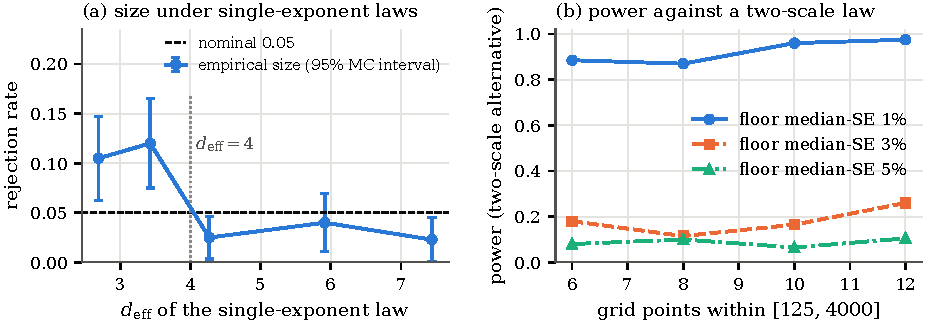
\includegraphics[width=\textwidth]{figures/fig_curvature_test.pdf}
\caption{The curvature test as a measuring instrument. (a) Rejection rate
against exact single-exponent laws with $95\%$ Monte-Carlo intervals: the
rate exceeds the nominal level below $\deff = 4$, where a single power law
is misspecified. (b) Power against a two-scale alternative as a function of
the number of grid points within $[125, 4\,000]$, at three floor
precisions.}
\label{fig:curvature-test}
\end{figure}

\subsection{Severity of a Non-Rejection}\label{sec:sizing-severity}

A non-rejection by a test of limited power does not establish that the
decay follows a single power law. What it does establish depends on the
precision of the floor, and we report it as a severity threshold in the
sense of the smallest departure the test would have detected.

\begin{defn}[Severity threshold]\label{def:severity}
For an admissible floor profile with fitted $(C, \deff)$ and a drift
factor $\delta \geq 1$, consider the alternative floor with exponents
$\deff\sqrt{\delta}$ on the lower half of $\mathcal{G}$ and
$\deff/\sqrt{\delta}$ on the upper half, joined at the midpoint of the
grid and perturbed by the measured noise of the profile. The
\emph{severity threshold} $\delta_{50}$ is the drift at which the
rejection probability of the curvature test equals $1/2$, obtained by
linear interpolation of Monte-Carlo rejection rates in $\log \delta$.
\end{defn}

Drifts below $\delta_{50}$ remain undetected at least half of the time, so
a non-rejection is informative only about departures larger than
$\delta_{50}$. The Monte-Carlo estimate of $\delta_{50}$ has two sources of
error: the binomial error of the rejection rates within one simulation
seed, and the variation of the whole procedure between seeds. We estimate
both from eight seeds and report a combined $90\%$ interval. On seven
of the eight admissible benchmark cells of \cref{sec:empirical} the
between-seed component is the larger of the two, and the combined interval
is $1.38$--$2.19\times$ wider than the binomial interval alone, with a median
of $1.65\times$.

\subsection{The Prescription as an Interval}\label{sec:sizing-interval}

Following \cref{prop:inversion}, we propagate the estimation error of the
fitted pair $(\log C, 1/\deff)$ through \cref{eq:requiredn}. We draw from a
multivariate $t$ distribution centred at the weighted least-squares estimate
with its estimated covariance and report quantiles of the resulting
prescriptions. The coverage of this interval was measured on exact power
laws with known parameters: at nominal level $0.90$ it delivers between
$0.860$ and $0.920$, with a median of $0.880$ slightly below the
nominal level. A calibrated version requests the nominal level $0.9125$,
which delivers $0.90$ as a median over the regime in which it was measured:
six-point grids over $[125, 4\,000]$, $n_{\mathrm{rep}} = 12$,
$d \in \{4, 5, 6\}$ and replicate coefficients of variation in
$\{0.03, 0.08, 0.13\}$. Away from this regime the calibration is not
applied, and the uncalibrated interval is returned with a flag; the regime
in which the software applies it is stated with every interval.

The coverage refers to independent replicate noise at each grid size. On
real data all grid sizes are subsampled from one table with shared random
numbers, which reduces the variance of the drift statistic to $0.81$ times
its value under independent replicates; the construction is therefore, if
anything, conservative on real data. The interval is conditional on the data
set at hand and does not describe how much a second data set from the same
law would change the answer. That variation is not negligible: on the
benchmark tables of \cref{sec:empirical}, the slope dimension estimate varies
$1.1$ to $2.1$ times more across half-size subsamples of a table than across
re-splits of the whole table, with a median of $1.5$.

% ==========================================================================
\section{Reporting an Evaluation}\label{sec:reporting}

A designed evaluation must also report its outcome on a scale that is
comparable across sample sizes and robust to degenerate generators. This
section defines such a scale and the associated tests.

\subsection{Reference Generators and the Skill Score}\label{sec:reporting-hierarchy}

A raw distance has no meaning on its own: a value of $0.1$ indicates an
excellent generator if the floor at that sample size is $0.09$ and a poor
one if it is $0.001$. We therefore compare every generator with reference
generators that are computed from the real data and require no training.
\begin{itemize}
\item \textbf{T0} places all mass at the real mean. Its distance to the
  real sample is the data scale $\tau$, and it is the best constant
  generator.
\item \textbf{T1} resamples each column independently. It reproduces all
  marginal distributions and no dependence between columns; it coincides
  with the \texttt{perm} reference of \citet{yang2024}.
\item \textbf{T2} is the Gaussian law with the real mean and covariance. It
  reproduces first and second moments and nothing beyond them.
\item \textbf{T$_{\mathrm{self}}$} resamples real observations that are not
  in the reference subsample, as the \texttt{self} reference of
  \citet{yang2024}. It approximates an ideal generator and serves as a
  ceiling. Drawn from the disjoint remainder, its distance is $1.07\times$ the floor; resampled from the whole data set, it falls below the floor, to $0.88\times$, because it shares observations with the reference (eight-dimensional Gaussian copula, $n = 500$, median over $20$ seeds).
\end{itemize}

\begin{defn}[Skill score]\label{def:skill}
Let $D_{\mathrm{obs}}$ be the distance between a generated sample and a real
reference sample of the same size $n$, let $f = f(n)$, and let $D_B$ be the
distance of a reference generator $B$. The \emph{floor-corrected ratio} is
\begin{equation}\label{eq:skill}
  V \;=\; \frac{D_{\mathrm{obs}} - f}{D_B - f},
\end{equation}
and the \emph{skill} relative to $B$ is $1 - V$.
\end{defn}

The skill equals $1$ for a generator that is as close to the real sample as
a second real sample, and $0$ for a generator as distant as the reference
$B$. Subtracting the floor from numerator and denominator makes $V$
dimensionless. For a fixed model law $Q \neq P$, $V \to \Wtwo(P,Q)/\Wtwo(P,Q_B)$
as $n \to \infty$, which does not depend on $n$, and for $Q = P$,
$V \to 0$; at finite $n$ the subtraction is a first-order correction, and
$V$ still varies with $n$. On an eight-dimensional Gaussian copula with non-Gaussian marginals at $n = 500$ per side, the median skill relative to T1 over $20$ seeds is $+1.00$ for a fresh draw from the true law (range $0.96$ to $1.03$), $+0.83$ for a sample of T2, $+0.00$ for a sample of T1 and $-0.52$ for a sample of T0.

\subsection{A Two-Sided Floor Test}\label{sec:reporting-twosided}

A one-sided test that asks only whether $D_{\mathrm{obs}}$ exceeds the floor
rewards a generator that returns the training observations. Such a sample
shares points with the reference sample, its distance falls below the
floor, and the one-sided test finds no evidence against it. On a
six-dimensional Gaussian copula, an exact copy of the training data obtains
a skill of $+1.42$ relative to T2, above the nominal maximum of $1$, whereas
a fresh draw from the true law obtains $+0.91$. \citet{chen2026} reports the
analogous phenomenon for image metrics.

If the generator draws fresh samples from $P$, $D_{\mathrm{obs}}$ is an
ordinary draw from the replicate distribution and should lie in neither of
its tails. We therefore report both tail probabilities,
$p_{\mathrm{hi}} = \Prob(D' \geq D_{\mathrm{obs}})$ and
$p_{\mathrm{lo}} = \Prob(D' \leq D_{\mathrm{obs}})$, where $D'$ follows the
replicate distribution, as Monte-Carlo $p$-values. A small $p_{\mathrm{hi}}$ indicates a generator
distinguishable from real data, and a small $p_{\mathrm{lo}}$ indicates a
sample that is closer to the reference than a second real sample would be,
the signature of leakage. A skill above $1$ is not itself evidence of
leakage: for a generator that draws from $P$, the probability of a skill
above $1$ is close to one half, $0.52$ at $d = 4$ and $0.42$ at $d = 8$ in
$200$ trials each, and a rule flagging $V < -0.05$ against T2 would flag
24--28\% of such generators. The lower-tail probability is the calibrated
statistic.

The skill score also needs its own interval, because its denominator
$D_B - f$ is itself random. On the numeric columns of \texttt{adult} at
$n = 250$, the standard deviation of $D_{\mathrm{T1}}$ across random seeds
is $0.222$, which is $13\times$ the difference $D_{\mathrm{T1}} - f = 0.017$
that forms the denominator.

\subsection{Null-Calibrated Leakage Screening}\label{sec:reporting-leakage}

A memorising generator produces a skill value that says nothing about
fidelity, so leakage screening is part of the evaluation. We split the real
sample into disjoint halves $A$ and $B$. Because $B$ is a genuine sample
from $P$ that shares no observation with $A$, the distribution of
distances from points of $B$ to their nearest neighbours in $A$, and the
fraction of exact duplicates, describe what a generator drawing fresh
samples from $P$ produces. The generated sample is compared with this null,
so the screen needs no threshold chosen in advance. It detects an exact
memoriser of a table with $60\,000$ rows and raises no alarm on any of four
same-law generators for discrete laws, where real observations
legitimately coincide.

Two limits apply to every screen of this kind. A memoriser that perturbs
each copied record by more than about $0.44\times$ the median distance
between records escapes detection. And when a law has a finite support that
the sample covers densely, so that $n/|\mathrm{support}| \approx 1$,
memorisation cannot be distinguished from fresh sampling by any detector,
including density-based membership-inference attacks that target local
overfitting \citep{vanbreugel2023}; the remedy is a training split
disjoint from the evaluation data.

\subsection{The Minimum Detectable Difference}\label{sec:reporting-mdd}

Let two generators be evaluated against the same real reference sample
$X_r$, with distances $D_A = D(X_r, Y_A)$ and $D_B = D(X_r, Y_B)$. Sharing
$X_r$ removes the variability of the reference from the difference
$D_A - D_B$.

\begin{defn}[Minimum detectable difference]\label{def:mdd}
At significance level $\alpha$ and power $1-\beta$, the \emph{minimum
detectable difference} at size $n$ is
\begin{equation}\label{eq:mdd}
  \MDD \;=\; \bigl(z_{1-\alpha/2} + z_{1-\beta}\bigr)\,
  \sigma_{\mathrm{pair}},
  \qquad
  \sigma_{\mathrm{pair}} = \sd\bigl(D(X_r, Y_A) - D(X_r, Y_B)\bigr),
\end{equation}
where the standard deviation is taken over independent draws of the
reference sample and of both generated samples of size $n$.
\end{defn}

Every detectability statement in this paper specifies both $\alpha$ and
the power. The common practice of calling a difference significant when it
exceeds two standard deviations corresponds to power $1/2$: in simulation,
a true difference equal to that threshold is detected with frequency $0.51$ over 400 trials, against $0.500$ analytically.

The paired standard deviation depends on the level of the distances being
compared, because the spread of $D$ grows with its mean. Before any model
exists it can be estimated in two ways. The \emph{direct estimate} draws
repeated real references and pairs of samples from a reference generator
at the level of interest, typically T1, and computes their standard
deviation. The \emph{floor proxy} scales the replicate variability of the
floor to that level, $\sqrt{2}\,\mathrm{CV}(f) \cdot D_{\mathrm{level}}$,
where $\mathrm{CV}(f)$ is the coefficient of variation of the replicate
distribution. The proxy requires no additional computation and overstates
the paired standard deviation: on a synthetic copula by factors between
$1.39$ and $1.75$ ($200$ replicates for each of three generators), and on the
benchmark tables of \cref{sec:empirical-atlas} by factors between $1.05$ and
$10.53$. Using the unscaled floor variability instead is not safe: its ratio
to the paired spread falls from $1.38$ near the floor to $0.79$ at the level
of T1, so it understates the spread where models are compared. Differences
between models are measured on the scale of $D$, which does not translate
linearly into differences between laws: shifting a law by a fixed vector
that raises the expected distance by one equivalence margin
(\cref{sec:reporting-tost}) changes the optimal matching and multiplies the
standard deviation of $D$ by $2.9$.

\subsection{Equivalence Testing}\label{sec:reporting-tost}

A statement that a generator is indistinguishable from real data is an
equivalence claim, and it requires an equivalence test. We apply the two
one-sided tests procedure \citep{westlake1981,schuirmann1987} to the
difference between $D_{\mathrm{obs}}$ and the floor, with a margin
$\eta$ fixed before the evaluation, and report $\eta_{\min}$, the
smallest margin that the precision of the floor can support. On a
six-dimensional copula, with the margin $\eta = 0.2193$ set to a quarter of
the floor and $\alpha = 0.05$, the
procedure declares equivalence at the boundaries $\pm\eta$ with
frequency $0.0$, so its size is at most $\alpha$; it declares equivalence
for fresh draws from the true law with frequency $1.0$; and it rejects the
memoriser, whose distance to the reference is zero. For $\eta = 0$ it
reduces to the two-sided floor test of \cref{sec:reporting-twosided}. The
upper-tail $p$-value is calibrated for fresh draws: over $200$ fresh generators, $\Prob(p_{\mathrm{hi}} \leq 0.05) = 0.045$ and the median is $0.524$. An
evaluation whose $\eta_{\min}$ exceeds every margin of interest cannot
establish equivalence for any generator; this is a property of its design.

\subsection{The Procedure in Brief}\label{sec:reporting-procedure}

\Cref{fig:procedure} collects the steps of
\cref{sec:floor,sec:sizing,sec:reporting} into one procedure. The design
steps use the real data only; the significance level, the power, the
equivalence margin and the embedding of categorical columns are fixed
before any generator is evaluated.

\begin{figure}[t]
\centering
\fbox{\begin{minipage}{0.93\textwidth}
\small
\textbf{Before any model is trained} (real data $X$ with $N$ rows)
\begin{enumerate}[label=\arabic*., leftmargin=1.6em, itemsep=2pt]
\item Fix $\alpha$, the power $1-\beta$, the equivalence margin $\eta$ and at
  least two embeddings of categorical columns (\cref{sec:discussion-mixed});
  standardise the columns on $X$.
\item Measure the floor on the grid $N/64, \dots, N/2$ with
  $n_{\mathrm{rep}} \geq 19$ disjoint splits, fit the floor law and run the
  curvature test (\cref{def:exponent,def:curvature}).
\item If the profile is admissible and $\deff \geq 4$, report the
  prescription interval (\cref{sec:sizing-interval}) and the severity
  threshold (\cref{def:severity}); otherwise report the range of the
  half-grid prescriptions.
\item Report the minimum detectable difference at the planned size, measured
  at the level of a reference generator or bounded by the floor proxy
  (\cref{def:mdd}).
\item For a latent-generative certificate, compare the slope estimate
  $\dhat$ and its tail index with the limit at $N$
  (\cref{sec:cert-crossings,sec:cert-transfer}).
\end{enumerate}
\textbf{After the models are trained}
\begin{enumerate}[resume*]
\item For each generated sample, report the distance, the skill against T0,
  T1 and T2 with its interval, both tail probabilities and the leakage
  screen (\cref{sec:reporting-hierarchy,sec:reporting-twosided,sec:reporting-leakage}).
\item Claim indistinguishability only through the equivalence test at the
  margin $\eta$ (\cref{sec:reporting-tost}), and state $\alpha$ and the power
  with every detectability statement.
\end{enumerate}
\end{minipage}}
\caption{Designing and reporting an evaluation based on $\Wtwo$.}
\label{fig:procedure}
\end{figure}

% ==========================================================================
\section{Limits of Latent-Generative Certificates}\label{sec:cert}

The preceding sections concern what an evaluation can measure. This section
concerns what it can prove about a latent-generative model, and shows that
the resolution floor limits both.

\subsection{Setting}\label{sec:cert-setting}

Let $\Ups$ be the data distribution on $\R^m$ and $\UpsN$ the empirical
measure of $N$ observations from it. A latent-generative model consists of a
latent law $\Sigma$ and a measurable decoder $g$; its output law is
$\UpsT = g_{\#}\Sigma$, and $\UpsTM$ is the empirical measure of $M$ decoded
latent draws. The certificates of \citet{dao2023} and \citet{lee2025} rest on
the triangle inequality
\begin{equation}\label{eq:decomp}
  \Wtwo(\Ups, \UpsT) \;\leq\;
  \underbrace{\Wtwo(\Ups, \UpsN)}_{\text{statistical term}} \;+\;
  \underbrace{\Wtwo(\UpsN, \UpsTM)}_{\text{empirical term}} \;+\;
  \underbrace{\Wtwo(\UpsTM, \UpsT)}_{\text{sampling term}} .
\end{equation}
The sampling term can be made small by drawing more latent samples. The
empirical term involves only finite samples and is usually bounded through
the Lipschitz constant of the decoder; \cref{sec:pullback} shows that it can be
bounded without that constant. The statistical term depends on the unknown
distribution $\Ups$ and on the number $N$ of available observations, and no
computation reduces it. Following \citet{dziugaite2017}, we call a bound
\emph{vacuous} when it is not smaller than the trivial bound, here the data
scale $\tau$ of $\Ups$.

\subsection{A Vacuity Criterion and a Computable Surrogate}\label{sec:cert-surrogate}

\begin{prop}[Vacuity criterion]\label{prop:vacuity}
Let $S = \Wtwo(\Ups, \UpsN)$ be the statistical term of \cref{eq:decomp}
and $\tau$ the data scale. If $S/\tau > 1$, then the right-hand side of
\cref{eq:decomp} exceeds $\tau$ and every bound of this form is vacuous.
\end{prop}

The statistical term cannot be computed, because it involves the
population. Its expected size is approximated by the distance between two
independent samples of size $N$ from the same law, which obeys the same rate
with a larger constant, heuristically by a factor $2^{1/d^*}$ that tends to
$1$ as $d^*$ grows. For a law of intrinsic dimension $d$ we therefore use
the dimensionless \emph{floor ratio}
\begin{equation}\label{eq:surrogate}
  r(d, N) \;=\; \frac{\E\, D(X_N, X'_N)}{\tau}
\end{equation}
as a surrogate for $\E\,S/\tau$. The triangle inequality gives $D(X_N, X'_N) \leq \Wtwo(\mu_N, P) + \Wtwo(P, \mu'_N)$ and hence only $\E\,S \geq r\,\tau/2$. The surrogate is closer than this bound suggests: on
isotropic Gaussian laws, the ratio of the two-sample distance to the
distance between a sample of size $N$ and a large reference sample lies
between $1.007$ and $1.16$, decreasing with $d$ and $N$
(\cref{app:details-two-sample}). The antecedent of \cref{prop:vacuity} is the
statistical term; a crossing of the surrogate implies a crossing of the
term up to this measured factor.

\subsection{Reference Tables}\label{sec:cert-table}

We measured $r(d, N)$ on isotropic Gaussian laws, for which the intrinsic
and the ambient dimension coincide and $\tau = \sqrt{d}$, with exact
transport and $20$ replicates per cell (\cref{tab:rsurface}). The ratio
rises with $d$, exceeds $1$ between $d = 16$ and $d = 64$, and decreases
slowly with $N$. The standard error of every cell is at most $0.0031$ for
$d \geq 4$ and at most $0.013$ overall. Near the crossing the sensitivity
$\mathrm{d}\log d / \mathrm{d}\log r$ is between $3.9$ and $5.5$, so a relative error $\varepsilon$ in $r$ shifts the crossing by a relative
amount of about $5\varepsilon$ in $d$; \cref{sec:empirical-margins} propagates this.

\begin{table}[htbp]
\centering
\small
\begin{adjustbox}{max width=\textwidth}
\begin{tabular}{lcccccccc}
\toprule
$d$ & 1 & 2 & 4 & 8 & 16 & 32 & 64 & 128 \\
\midrule
$N = 256$ & 0.158 & 0.236 & 0.435 & 0.681 & 0.895 & 1.052 & 1.161 & 1.239 \\
$N = 1\,024$ & 0.075 & 0.137 & 0.315 & 0.568 & 0.804 & 0.986 & 1.117 & 1.208 \\
$N = 2\,048$ & 0.052 & 0.107 & 0.268 & 0.519 & 0.765 & 0.957 & 1.097 & 1.194 \\
$N = 4\,096$ & 0.037 & 0.078 & 0.227 & 0.475 & 0.729 & 0.931 & 1.078 & 1.180 \\
$N = 8\,192$ & 0.031 & 0.059 & 0.191 & 0.435 & 0.694 & 0.905 & 1.060 & 1.168 \\
$N = 16\,384$ & 0.021 & 0.044 & 0.162 & 0.399 & 0.662 & 0.880 & 1.042 & 1.156 \\
$N = 32\,768$ & 0.013 & 0.033 & 0.137 & 0.366 & 0.631 & 0.857 & 1.025 & 1.144 \\
\bottomrule
\end{tabular}
\end{adjustbox}
\caption{The floor ratio $r(d, N)$ of \cref{eq:surrogate} on isotropic
Gaussian laws of dimension $d$ with $N$ observations per side (exact
transport, $20$ replicates per cell).}\label{tab:rsurface}
\end{table}

\subsection{Crossings in the Units of a Measured Dimension}\label{sec:cert-crossings}

On isotropic laws, $r(d, N)$ crosses $1$ at nominal dimension
$d \approx 25.8$, $34.6$, $39.9$, $44.9$, $49.6$, $54.0$ and $58.2$ for $N = 256$,
$1\,024$, $2\,048$, $4\,096$, $8\,192$, $16\,384$ and $32\,768$. A practitioner does not know the nominal
dimension of real data; the available quantity is a measured estimate such
as the slope estimate $\dhat$ of \cref{def:dhat}. This estimate is biased
upward in low dimension and downward in high dimension: nominal dimension
$64$ is measured as $36.4$ at $N = 2\,048$ and $41.0$ at $N = 32\,768$.
Comparing a measured estimate with a threshold stated in nominal units
therefore overstates the available headroom: at the crossings below, the
nominal limit exceeds the measured one by factors between $1.50$ and
$1.54$.
We tabulated the mean of $\dhat$ on the same isotropic laws
(\cref{tab:dhat} in \cref{app:details-tables}) and map the crossing into
measured units. The resulting limits are
$\dhat \approx 17.2$ $[16.6, 17.8]$ at $N = 256$,
$22.8$ $[22.1, 23.6]$ at $N = 1\,024$,
$26.0$ $[25.5, 26.4]$ at $N = 2\,048$,
$29.6$ $[29.3, 30.0]$ at $N = 4\,096$,
$32.3$ $[32.1, 32.5]$ at $N = 8\,192$ and
$35.2$ $[35.0, 35.4]$ at $N = 16\,384$ and
$38.3$ $[38.0, 38.5]$ at $N = 32\,768$,
where the $90\%$ intervals propagate the sampling error of both tables
(\cref{fig:reference-tables}). A data set whose measured dimension exceeds the limit for
its size admits no informative certificate of the form \cref{eq:decomp}.
The tables cover $N \leq 32\,768$. For larger $N$ the software clamps the
limit at its value for $32\,768$, which understates the true limit.

\begin{figure}[t]
\centering
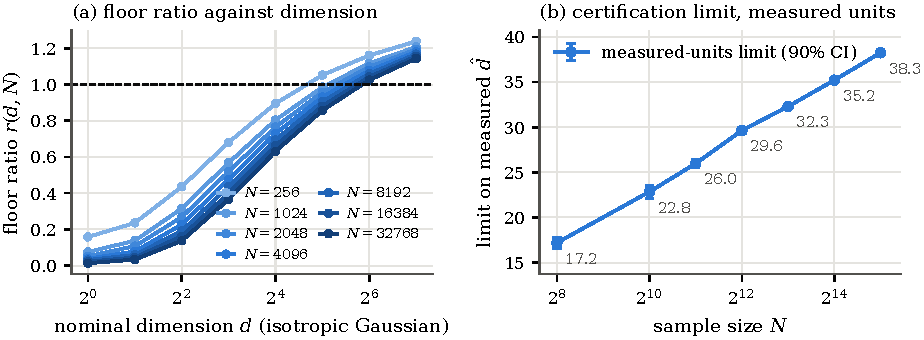
\includegraphics[width=\textwidth]{figures/fig_reference_tables.pdf}
\caption{(a) The floor ratio $r(d, N)$ on isotropic Gaussian laws for
$N = 256$ to $32\,768$ observations per side; the dashed line is the trivial
scale $r = 1$. (b) The resulting certification limit in the units of the
slope dimension estimate, with $90\%$ intervals propagating the sampling
error of both reference tables.}
\label{fig:reference-tables}
\end{figure}

\subsection{Transfer to Other Classes of Laws}\label{sec:cert-transfer}

The reference tables are built on isotropic Gaussian laws, and applying them
to real data requires that $r$ depend on the law mainly through its measured
dimension. We tested this on three families of non-isotropic laws in
$64$ ambient dimensions, namely anisotropic Gaussians, factor models and
curved manifolds (\cref{app:details-transfer}), with measured dimensions
$\dhat \approx 9.7$--$22.8$, the band in which the crossing lies. Indexed by
the measured dimension, the isotropic table predicts the measured floor
ratio with a median residual of $-0.4\%$ and a range of $-9.9\%$ to $+7.2\%$.
The isotropic reference itself, measured with three replicates, varies
between $-7.5\%$ and $+7.0\%$, so the residuals are within its own
measurement noise.

These three families are smooth, unimodal and light-tailed. We tested two
further classes, with a verdict rule fixed before the experiment: a class
transfers if every residual in the band lies within $\pm 12\%$, the range
above widened by the reference noise. Lattice laws transfer: factor models
rounded to a grid of step $0.5$ or $1$ in every coordinate give residuals
between $-8.7\%$ and $+2.6\%$, and rounding half of the coordinates gives
$-5.0\%$ and $-4.3\%$. In $64$ dimensions these lattices produce no
coincident observations, so the test does not cover coarse low-dimensional
lattices such as integer-coded categorical columns, where ties reduce the
floor (\cref{app:proofs}, remark after the proof of \cref{prop:floor}).
Polynomial tails do not transfer: a multivariate Student-$t$ law with
$\nu = 3$ degrees of freedom gives a residual of $+44.1\%$ at $N = 1\,024$,
and at $N = 256$ its dimension cannot be estimated. With $\nu = 5$ the
residuals are $+6.3\%$ in the band and $-13.7\%$ outside it, and a rotated
Laplace law with exponential tails stays within $\pm 1\%$. A positive
residual means that the table understates $r$, so the certification limit is
optimistic for polynomially tailed laws.

We therefore report, with every dimension estimate, the Hill estimate \citep{hill1975} of the tail index of the distances from the median, computed from the largest
$5\%$ of those distances, and flag values below $5$. On the probe laws the
estimate is $2.8$ for $\nu = 3$, $4.4$ for $\nu = 5$, $9.0$ for the Laplace
law and $16.1$ for an anisotropic Gaussian. The flag is a screening device
without a formal guarantee. It is raised on eight of the eleven benchmark
cells of \cref{sec:empirical}, whose estimates range from $2.75$ to
$10.94$; \cref{sec:empirical-margins} accounts for this.

% ==========================================================================
\section{A Certificate Without a Lipschitz Constant}\label{sec:pullback}

The empirical term of \cref{eq:decomp} compares decoded samples. Published
certificates bound it by the latent transport distance multiplied by a
Lipschitz constant of the decoder. This section shows that the constant is
unnecessary for the empirical statement and that removing it tightens the
bound substantially.

\subsection{The Plan-Pullback Bound}\label{sec:pullback-bound}

\begin{lem}[Pushforward coupling]\label{lem:pushforward}
Let $\Sigma$ and $\Sigma'$ be Borel probability measures on a latent space, let
$\pi \in \Pi(\Sigma, \Sigma')$, and let $g$ be a measurable map into $\R^{m}$
with $\int \|g(z)\|^2 \,\mathrm{d}\Sigma(z) < \infty$ and
$\int \|g(z)\|^2 \,\mathrm{d}\Sigma'(z) < \infty$. Then $(g \otimes g)_{\#}\pi$ is a
coupling of $g_{\#}\Sigma$ and $g_{\#}\Sigma'$, and consequently
\begin{equation}\label{eq:lemma}
  \Wtwo\bigl(g_{\#}\Sigma,\, g_{\#}\Sigma'\bigr)^{2} \;\leq\;
  \int \bigl\| g(z) - g(z') \bigr\|^{2} \, \mathrm{d}\pi(z, z').
\end{equation}
\end{lem}

\Cref{lem:pushforward} is elementary \citep[Chapter~1]{villani2009}; we
prove it in \cref{app:proofs}. The Lipschitz certificate follows from
\cref{eq:lemma} by bounding the integrand by $L^{2}\|z - z'\|^{2}$, where $L$
is a Lipschitz constant of $g$, and choosing $\pi$ optimal for the latent
cost. For empirical measures this bounding step can be omitted.

\begin{prop}[Empirical plan-pullback bound]\label{prop:ppc}
Let $\sigma^{*}$ be an optimal assignment, for the squared Euclidean cost,
between latent points $z_1, \dots, z_N$ and $z'_1, \dots, z'_N$ with uniform
empirical measures $\Sigma_N$ and $\Sigma'_N$. Then, for every measurable
decoder $g$,
\begin{equation}\label{eq:lemma-empirical}
  \Wtwo\bigl(g_{\#}\Sigma_{N},\, g_{\#}\Sigma'_{N}\bigr)^{2} \;\leq\;
  \frac{1}{N} \sum_{i=1}^{N}
  \bigl\| g(z_i) - g(z'_{\sigma^{*}(i)}) \bigr\|^{2},
\end{equation}
and the right-hand side can be evaluated exactly with $2N$ evaluations of $g$.
\end{prop}

\Cref{prop:ppc} applies when both samples consist of decoded latent points,
as when the observations are represented by their encodings: with
$\Sigma_N$ the empirical measure of the encoded observations and $\Sigma'_N$ that
of $N$ latent draws, the left-hand side of \cref{eq:lemma-empirical} is the
empirical term of \cref{eq:decomp} computed on reconstructions.

The bound holds for every decoder because $\sigma^{*}$ defines a valid
coupling of the decoded samples, although not necessarily an optimal one.
It needs no derivative of $g$ and no Lipschitz constant. The Lipschitz step is also the expensive one: exact computation of a network's Lipschitz constant is NP-hard
\citep{virmaux2018}, the product of the layer spectral norms
\citep{szegedy2014} is a loose upper bound, and tighter bounds require
semidefinite relaxations \citep{fazlyab2019}. Optimality of $\sigma^{*}$ is
not needed for validity; it makes the bound tight when $g$ approximately
preserves the latent geometry.

\subsection{Tightness on Trained Decoders}\label{sec:pullback-tightness}

For empirical measures of equal size the left-hand side of
\cref{eq:lemma-empirical} is itself an assignment problem and can be
computed exactly, so the tightness of the bound is a measurable quantity.
We trained variational autoencoders \citep{kingma2014} on the
\texttt{digits} data set of the UCI repository \citep{kelly2026}, as
distributed with scikit-learn \citep{pedregosa2011} ($1\,797$ observations of
dimension $64$), using $1\,300$ observations for
training, in two architectures and with three training seeds each
(\cref{app:details-vae}). For each trained model and each of two evaluation
draws, we compared the encoder means of $400$ held-out observations with
$400$ draws from the latent prior, both decoded by the trained decoder.

Across these twelve cells, the plan-pullback bound is $1.07$--$1.15\times$ the
exact output-space distance, with a median of $1.09\times$, and never falls
below it (\cref{fig:pullback}). The certificate obtained from the product of the
decoder's layer spectral norms is $12$--$120\times$ the exact distance, with a
median of $53\times$. Replacing the certified constant by the largest
Lipschitz ratio observed between sampled latent pairs, which is a lower
bound on the true constant and no longer yields a valid certificate, still
gives $1.8$--$5.1\times$, with a median of $2.9\times$. Most of the looseness of
the Lipschitz route therefore comes from replacing the cost of an actual
coupling by a worst-case stretch factor, and only part of it from the
looseness of the spectral-norm product.

\begin{figure}[t]
\centering
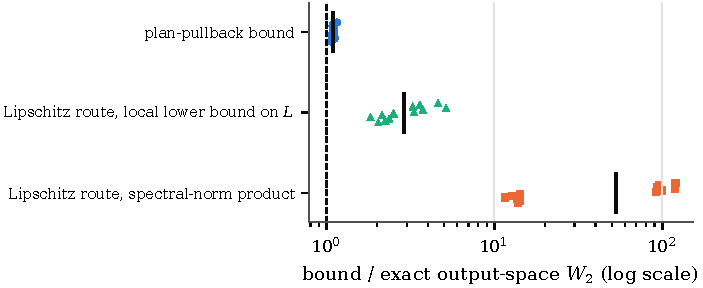
\includegraphics[width=0.62\textwidth]{figures/fig_plan_pullback.pdf}
\caption{Bounds on the output-space $\Wtwo$ between decoded held-out
encodings and decoded prior draws, divided by the exact distance (log
scale). Twelve cells: two architectures, three training seeds and two
evaluation draws; vertical bars mark medians. The plan-pullback bound of
\cref{prop:ppc} is valid in every cell; the Lipschitz certificate uses the
product of spectral norms; the middle row uses a sampled lower bound on the Lipschitz constant and is not a valid certificate.}
\label{fig:pullback}
\end{figure}

\subsection{Scope}\label{sec:pullback-scope}

\Cref{prop:ppc} bounds the distance between decoded samples that have been
drawn. A Lipschitz constant remains necessary for statements about latent
points that have not been drawn, such as a guarantee that holds uniformly
over the latent space, and for outputs too expensive to decode. The
tightness figures above are measurements on one data set with two
architectures; the validity of the bound holds for every decoder.

% ==========================================================================
\section{Empirical Study on Tabular Benchmarks}\label{sec:empirical}

We apply the procedures of \cref{sec:floor,sec:sizing,sec:reporting,sec:cert}
to public tabular benchmarks, using the real data alone.

\subsection{Data and Protocol}\label{sec:empirical-design}

We analysed nine public data sets: \texttt{adult},
\texttt{census-income} and \texttt{shuttle} from the UCI Machine Learning
Repository \citep{kelly2026}, \texttt{bank-marketing} \citep{moro2014},
\texttt{covertype} \citep{blackard1999}, \texttt{higgs} \citep{baldi2014},
\texttt{letter} \citep{frey1991}, \texttt{MagicTelescope}
\citep{bock2004} and \texttt{pendigits} \citep{alimoglu1997}. All except
\texttt{covertype} were obtained from OpenML \citep{vanschoren2014}, and
\texttt{covertype} through scikit-learn \citep{pedregosa2011}; the
identifiers, versions and checksums of the downloaded tables, and a digest
of every encoded matrix, are stored with the results. Each data set is
represented by up to two encodings. Encoding E1
keeps the numeric columns; encoding E2 adds the categorical columns as
integer codes. Where a data set has no categorical columns, or where the two
encodings coincide, as for \texttt{covertype}, one cell is reported, which
gives eleven table--encoding cells. For each cell we standardised the
columns and drew $8\,000$ rows at random (seed $0$). Floors were computed by
exact assignment on the six-point grid $\{125, 250, \dots, 4\,000\}$ with
$n_{\mathrm{rep}} = 12$.

Three further candidate data sets were excluded by a screening step that
precedes the analysis, because the premise of the floor law fails on them.
On \texttt{electricity} \citep{gama2004}, a non-stationary series, the
floor does not decrease with $n$: the median distances are
$0.986/1.170/0.967$ at $n = 1\,000/2\,000/4\,000$. On
\texttt{eeg-eye-state} \citep{kelly2026}, recording artefacts reach
$89.4$ standard deviations and dominate the tails, and the floor medians are
not monotone in $n$: the median distance jumps from $0.975$ at $n = 1\,000$ to
$5.32$ at $n = 2\,000$. On \texttt{MiniBooNE} \citep{roe2005}, the floor medians are not
monotone in $n$, and a single power law has $R^2 = 0.59$.

For each cell we also report three dimension estimates: the slope estimate
of \cref{def:dhat}, averaged over eight re-splits; the TwoNN estimator of
\citet{facco2017}; and the maximum-likelihood estimator of
\citet{levina2004} with $10$ neighbours, in the form that \citet{pope2021}
applied to image data, which averages the inverses of the local estimates. Their \emph{spread}, the ratio of the largest to the smallest estimate,
indicates disagreement between the geometric and the transport-based view
of the data.

\subsection{Floor Laws}\label{sec:empirical-floor-laws}

\Cref{tab:floor-laws} and \cref{fig:floor-laws} report the fitted floor laws.
On eight of the eleven cells a single power law describes the floor: the
coefficient of determination is at least $0.984$, the curvature test
does not reject, with $p$-values of 0.112--0.995, and the exponents
range from $4.07$ to $13.24$, all in the dimension-governed
regime. The curvature test rejects a single exponent on \texttt{adult:E2}
and \texttt{covertype} ($p = 0.032$ and $0.042$), and the floor of
\texttt{shuttle:E1} admits no power law.

\begin{table}[htbp]
\centering
\small
\begin{tabular}{lcccccc}
\toprule
cell & $\deff$ & $R^{2}$ & curvature $p$ & admissible &
$\dhat \pm \mathrm{sd}$ & spread \\
\midrule
adult:E1 & 4.07 & 0.984 & 0.486 & yes & $4.48 \pm 0.96$ & 1.94$\times$ \\
adult:E2 & 5.91 & 0.998 & 0.032 & no & $5.79 \pm 0.31$ & 1.43$\times$ \\
bank-marketing:E1 & 4.85 & 0.993 & 0.955 & yes & $5.05 \pm 1.15$ & 1.20$\times$ \\
bank-marketing:E2 & 6.55 & 0.998 & 0.995 & yes & $6.20 \pm 0.71$ & 1.23$\times$ \\
census-income:E1 & 5.51 & 0.992 & 0.678 & yes & $5.18 \pm 1.44$ & 2.14$\times$ \\
covertype:E1=E2 & 5.42 & 0.975 & 0.042 & no & $4.64 \pm 0.48$ & 1.32$\times$ \\
higgs:E1 & 13.24 & 0.999 & 0.935 & yes & $13.31 \pm 0.51$ & 1.08$\times$ \\
letter:E1 & 5.34 & 0.999 & 0.596 & yes & $5.25 \pm 0.15$ & 1.10$\times$ \\
MagicTelescope:E1 & 5.59 & 0.997 & 0.172 & yes & $5.48 \pm 0.32$ & 1.26$\times$ \\
pendigits:E1 & 4.57 & 0.998 & 0.112 & yes & $4.83 \pm 0.33$ & 1.29$\times$ \\
shuttle:E1 & 9.45 & 0.591 & --- & no & $11.62 \pm 19.00$ & 7.25$\times$ \\
\bottomrule
\end{tabular}
\caption{Floor laws of the eleven benchmark cells ($8\,000$ rows,
six-point grid over $[125, 4\,000]$, $n_{\mathrm{rep}} = 12$). $\deff$ and
$R^2$ refer to the fit of \cref{def:exponent}; admissibility is decided by
the curvature test of \cref{def:curvature}; $\dhat$ is the slope estimate
with its standard deviation over re-splits; spread is the ratio of the
largest to the smallest of the three dimension estimates.}\label{tab:floor-laws}
\end{table}

\begin{figure}[htbp]
\centering
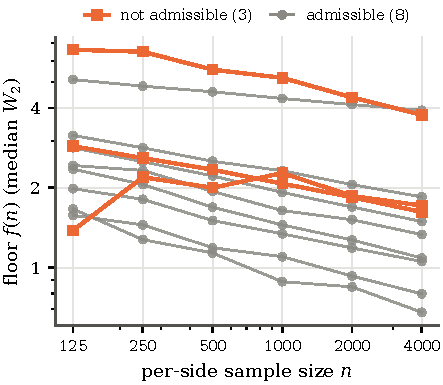
\includegraphics[width=0.55\textwidth]{figures/fig_floor_laws.pdf}
\caption{Measured floors $f(n)$ of the eleven benchmark cells on
logarithmic axes. Eight cells follow a single power law; the three cells
that are not admissible are drawn with squares.}\label{fig:floor-laws}
\end{figure}

The floor of \texttt{shuttle:E1} admits no power law at all. Its coefficient
of determination is $0.591$, the coefficient of variation of its
replicates reaches $1.60$ at $n = 125$, and its floor medians over
the grid,
\[
  1.38/2.19/2.00/2.27/1.86/1.71,
\]
are not monotone: over the lower half of the grid the floor increases with
$n$, so neither the curvature test nor the half-grid prescriptions are
defined. No prescription is returned for this cell. Computed nevertheless,
the $90\%$ interval of the full-grid prescription spans factors of
$53.4\times$ and $2108\times$ at the two targets of
\cref{sec:empirical-scope}. The dimension estimators agree with this
verdict: their spread is $7.25\times$, against
$1.08$--$2.14\times$ on the admissible cells, with the TwoNN and
maximum-likelihood estimators at $1.60$ and $2.02$ and the slope estimate at
$11.62$.

\subsection{Scope of the Sizing Rule}\label{sec:empirical-scope}

\Cref{tab:scope} reports, for every cell, the agreement between the
prescriptions of the two half-grid fits, the curvature $p$-value and the
severity threshold of \cref{def:severity} with its combined interval.

\begin{table}[htbp]
\centering
\small
\begin{tabular}{lcccc}
\toprule
cell & half-fit ratio & curvature $p$ &
$\delta_{50}$ [$90\%$ interval] & observed drift \\
\midrule
adult:E1 & 1.40$\times$ & 0.486 & 1.88 [1.72, 2.05] & below \\
adult:E2 & 1.51$\times$ & 0.032 & 1.19 [1.16, 1.21] & above \\
bank-marketing:E1 & 1.36$\times$ & 0.955 & 1.48 [1.41, 1.56] & below \\
bank-marketing:E2 & 1.18$\times$ & 0.995 & 1.20 [1.17, 1.23] & below \\
census-income:E1 & 1.35$\times$ & 0.678 & 1.86 [1.76, 1.97] & below \\
covertype:E1=E2 & 2.38$\times$ & 0.042 & 1.61 [1.54, 1.67] & above \\
higgs:E1 & 1.10$\times$ & 0.935 & 1.18 [1.17, 1.20] & below \\
letter:E1 & 1.18$\times$ & 0.596 & 1.13 [1.11, 1.14] & below \\
MagicTelescope:E1 & 1.37$\times$ & 0.172 & 1.28 [1.24, 1.33] & below \\
pendigits:E1 & 1.29$\times$ & 0.112 & 1.19 [1.16, 1.21] & below \\
shuttle:E1 & --- & --- & --- & --- \\
\bottomrule
\end{tabular}
\caption{Scope of the sizing rule. Half-fit ratio: largest ratio between the
prescriptions of the low-half and high-half fits. $\delta_{50}$: severity
threshold (\cref{def:severity}) with its combined binomial and between-seed
$90\%$ interval over eight seeds. Last column: position of the observed
drift of the cell relative to that interval.}\label{tab:scope}
\end{table}

Four results follow. First, the non-rejections bound the undetectable drift
at $\delta_{50} \leq 1.88\times$ on every admissible cell and at $1.13$ on the
most precisely measured one, \texttt{letter:E1}. Second, the observed drift
of every admissible cell lies below its $50\%$-detection interval, whereas on
the two cells the test rejects, \texttt{adult:E2} and \texttt{covertype}, it
lies above: their curvature is of a size the test detects more than half of
the time. Third, on the admissible cells the prescriptions of the two halves
of one grid agree within a factor of $1.10$--$1.40$, with a median of
$1.32$. Fourth, the $90\%$ interval of the prescription is
$1.07$--$2.04\times$ wide at the target $n = 10\,000$ and
$1.15$--$2.88\times$ at $n = 40\,000$, targets that lie $2.5\times$ and
$10\times$ beyond the largest grid size. Within these limits the sizing
rule is identified to within a factor of two to three on these tables. The
intervals widen with the distance of the target from the grid, as
\cref{prop:inversion} predicts.

\subsection{The Resolution Atlas}\label{sec:empirical-atlas}

The resolution atlas answers, for each benchmark and sample size and
without training any model, the question posed in the introduction: how
large must a difference in skill be before an evaluation can detect it?

\paragraph{Definition.} For a cell (table, $n$), let $f(n)$ be the floor
and $D_{\mathrm{T1}}$ the distance of the independent-columns reference T1
to a fresh real sample of the same size. The difference
$S = D_{\mathrm{T1}} - f$ is the \emph{skill range}: by \cref{def:skill} a
difference $\Delta D$ in distance corresponds to a difference $\Delta D / S$
in skill relative to T1. The \emph{resolvable skill difference} is
\begin{equation}\label{eq:atlas}
  \rho(n) \;=\; \frac{\bigl(z_{0.975} + z_{0.80}\bigr)\,
  \sigma_{\mathrm{pair}}}{D_{\mathrm{T1}} - f},
\end{equation}
the minimum detectable difference of \cref{def:mdd} at $\alpha = 0.05$ and
power $0.80$, expressed as a fraction of the skill range. We measured
$\sigma_{\mathrm{pair}}$ directly at the level of T1: in each of $30$
replicates we drew a fresh real reference of $n$ rows and two independent
samples of T1, and took the standard deviation of the difference of their
distances to the reference. A value $\rho = 1$ means that one minimum
detectable difference spans the whole range between a generator that
discards every dependence between columns and a generator as close to the
data as a second real sample. Protocol details are given in
\cref{app:details-atlas}.

\paragraph{Results.} \Cref{tab:atlas} and \cref{fig:atlas} report the
atlas for eight admissible table--encoding pairs and five sample sizes,
$n \in \{250, 500, 1\,000, 2\,000, 4\,000\}$. Over these $40$ cells, $\rho$
ranges from $0.014$ to $42.124$, with a median of $0.236$, and $40\%$ of the
cells have $\rho \geq 1$.

\begin{table}[htbp]
\centering
\small
\begin{adjustbox}{max width=\textwidth}
\begin{tabular}{lcccccc}
\toprule
& \multicolumn{3}{c}{$n = 4\,000$} & median of $\rho$ & proxy / & cells with span \\
\cmidrule(lr){2-4}
table & proxy & measured $\rho$ & $90\%$ interval & over $n$ & measured SD & inside noise \\
\midrule
bank-marketing:E1 & 8.543 & 4.488 & [3.705, 5.743] & 14.760 & 1.39 & 3 \\
adult:E1          & 5.041 & 3.526 & [2.911, 4.512] & 3.526 & 1.43 & 3 \\
bank-marketing:E2 & 1.799 & 0.764 & [0.630, 0.977] & 1.452 & 2.36 & 0 \\
census-income:E1  & 0.820 & 0.221 & [0.182, 0.283] & 0.596 & 2.58 & 0 \\
higgs:E1          & 0.068 & 0.065 & [0.053, 0.083] & 0.150 & 1.75 & 0 \\
MagicTelescope:E1 & 0.079 & 0.026 & [0.022, 0.034] & 0.056 & 3.70 & 0 \\
letter:E1         & 0.071 & 0.015 & [0.012, 0.019] & 0.044 & 3.23 & 0 \\
pendigits:E1      & 0.138 & 0.014 & [0.011, 0.018] & 0.037 & 7.72 & 0 \\
\midrule
\textit{shuttle:E1} & 3.419 & 1.806 & [1.491, 2.311] & 1.806 & 2.75 & 2 \\
\textit{covertype:E1} & 0.955 & 0.288 & [0.238, 0.369] & 1.271 & 1.89 & 1 \\
\textit{adult:E2} & 0.349 & 0.150 & [0.124, 0.192] & 0.237 & 2.30 & 0 \\
\bottomrule
\end{tabular}
\end{adjustbox}
\caption{The resolution atlas: the smallest resolvable difference in skill
relative to T1, in units of the skill range (\cref{eq:atlas}; $\alpha = 0.05$,
80\% power), for $n \in \{250, 500, 1\,000, 2\,000, 4\,000\}$ per side.
``Measured'' uses the paired standard deviation measured with $30$
replicates, with a $90\%$ interval from the $\chi^{2}$ law of the sample
standard deviation; ``proxy'' uses the floor proxy of
\cref{sec:reporting-mdd}. The last column counts the sample sizes at which
the skill range is smaller than the seed-to-seed standard deviation of
$D_{\mathrm{T1}}$; the column before it gives the median ratio of the proxy
to the measured paired standard deviation. Rows are ordered by the measured value at $n = 4\,000$;
the three cells that are not admissible (italic) are shown for completeness
and excluded from all summaries.}\label{tab:atlas}
\end{table}

\begin{figure}[htbp]
\centering
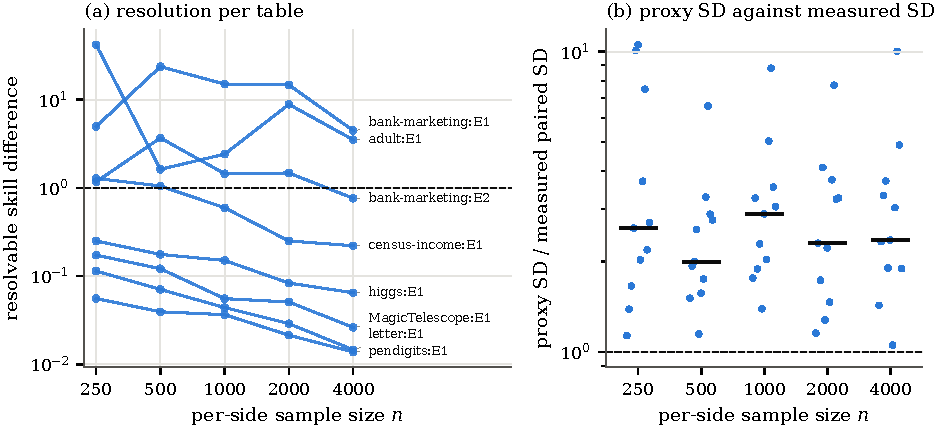
\includegraphics[width=\textwidth]{figures/fig_resolution_atlas.pdf}
\caption{The resolution atlas. (a) Smallest resolvable skill difference
$\rho$ against the per-side sample size, one line per admissible
table--encoding pair; the dashed line marks $\rho = 1$, where one minimum
detectable difference equals the whole skill range. (b) Ratio of the floor
proxy to the measured paired standard deviation for all $55$ cells; bars
mark medians.}\label{fig:atlas}
\end{figure}

Resolution varies strongly between benchmarks. At $n = 4\,000$ the
resolvable difference spans more than two orders of magnitude. On
\texttt{letter}, \texttt{pendigits} and \texttt{MagicTelescope}, a difference
of $1.4$--$2.6\%$ of the skill range is detectable. On \texttt{adult:E1} and
\texttt{bank-marketing:E1}, one minimum detectable difference is at least
$1.6$ times the whole skill range at every sample size measured, so on these
encodings no difference between generators can be resolved with $\Wtwo$ at
these sizes. The ordering follows the amount of dependence that T1 removes:
across the $40$ cells the Spearman rank correlation between the relative
skill range $(D_{\mathrm{T1}} - f)/f$ and $\rho$ is $-0.85$. Cells of one
table are not independent, so the coefficient is descriptive.

In six admissible cells the skill range is smaller than the seed-to-seed
standard deviation of $D_{\mathrm{T1}}$: \texttt{adult:E1} at $n = 250$,
$1\,000$ and $2\,000$, and \texttt{bank-marketing:E1} at $n = 250$, $500$
and $4\,000$. The same holds for two cells that are not admissible,
\texttt{covertype:E1} at $n = 500$ and \texttt{shuttle:E1} at $500$ and
$1\,000$. At these sizes an evaluation cannot detect that a generator has removed
every dependence in the table. For \texttt{adult:E1} the reason is visible
in the data: its six numeric columns have a largest pairwise absolute
correlation of $0.155$ and a median of $0.057$, so there is little
dependence to remove, and removing it changes $\Wtwo$ very little.

The floor proxy of \cref{sec:reporting-mdd} exceeds the measured paired
standard deviation in all $55$ cells, by factors between $1.05$ and $10.53$
with a median of $2.36$ (\cref{fig:atlas}b). It is therefore a conservative
substitute when the direct measurement is too expensive, and it can
overstate the required difference several-fold.

\paragraph{Scope.} The atlas concerns $\Wtwo$ at $n \leq 4\,000$ per side.
Marginal statistics, downstream-task scores and kernel tests can have
higher power against specific departures; $\Wtwo$ is an omnibus joint
distance, and omnibus tests lose power as the dimension grows. Encoding E1
is numeric only and E2 embeds categorical columns as integers, so neither is
a canonical representation of a mixed-type table (\cref{sec:discussion}).
The paired standard deviation of a single cell rests on $30$ replicates and
is determined to within roughly $-17\%$ and $+28\%$; conclusions are drawn
from the pattern across cells. Finally, every quantity here holds the
generator fixed and varies only the samples. Retraining a generator adds
variability, which \citet{dufour2026} found to be $3.2\times$ larger than
the resampling variability for image models, so the atlas gives lower
bounds on the differences required when trained models are compared.

\subsection{Certification Margins}\label{sec:empirical-margins}

Every admissible cell has a measured dimension of at most $13.31$, below
the certification limits of $26.0$ at $N = 2\,048$ and $29.6$ at
$N = 4\,096$ that bracket the $4\,000$ observations per side of these tables.
To quantify the margin, we propagated three sources of uncertainty jointly
by Monte Carlo with $8\,000$ draws per table: the sampling uncertainty of
$\dhat$ estimated by subsampling, a law-to-law residual in $r$ resampled from
the transfer study of \cref{sec:cert-transfer}, and the sampling error of the
calibration map of \cref{sec:cert-crossings} (\cref{app:details-margins}).
The margin in dimension units is the ratio of the crossing to the drawn
dimension, and the margin in $r$ units is $1/r$ at the drawn dimension, the
quantity that decides vacuity. \Cref{tab:margins} reports the fifth
percentiles for the eight admissible cells.

\begin{table}[htbp]
\centering
\small
\begin{tabular}{lcccc}
\toprule
cell & $\dhat$ & $q_{0.05}$, dimension units & $q_{0.05}$, $r$ units & $q_{0.05}$, $r$ units, heavy tails \\
\midrule
pendigits:E1       & 4.83 & $6.92\times$ & $3.23\times$ & $2.24\times$ \\
letter:E1          & 5.25 & $6.40\times$ & $3.08\times$ & $2.13\times$ \\
MagicTelescope:E1  & 5.48 & $5.92\times$ & $2.70\times$ & $1.87\times$ \\
bank-marketing:E1  & 5.05 & $5.91\times$ & $2.54\times$ & $1.77\times$ \\
adult:E1           & 4.48 & $5.84\times$ & $2.45\times$ & $1.70\times$ \\
census-income:E1   & 5.18 & $5.47\times$ & $2.32\times$ & $1.61\times$ \\
bank-marketing:E2  & 6.20 & $4.98\times$ & $2.18\times$ & $1.52\times$ \\
higgs:E1           & 13.31 & $2.13\times$ & $1.30\times$ & $0.90\times$ \\
\bottomrule
\end{tabular}
\caption{Certification margins of the eight admissible cells with three
sources of uncertainty propagated jointly ($8\,000$ Monte-Carlo draws per
cell, reference tables evaluated at the cells' own sample size). No draw
was vacuous in any cell, which bounds the probability of vacuity by about
$3/8\,000$ at $95\%$ confidence \citep{hanley1983}. The last column divides the $r$-unit margin by $1.441$, which
charges the largest heavy-tail residual of \cref{sec:cert-transfer} in
full.}\label{tab:margins}
\end{table}

The fifth-percentile margins in $r$ units range from $1.30\times$ to
$3.23\times$, and no draw was vacuous. Margins in dimension units are larger
because the crossing responds weakly to $r$ (\cref{sec:cert-table}); the
$r$ units are the relevant ones. Eight of the eleven cells are flagged as
heavy-tailed, and the last column therefore charges the $+44.1\%$ residual
of the Student-$t$ law in full. Seven cells keep a margin above one, between
$1.52\times$ and $2.24\times$. The exception is \texttt{higgs:E1}, whose
measured dimension of $13.31$ is the largest of the study and whose tail
index of $3.65$ is below the threshold: if its floor ratio carried the full
heavy-tail error, its fifth-percentile margin would be $0.90\times$ and a
certificate could not be ruled informative. With this exception, the
statistical term does not rule out certificates of the form
\cref{eq:decomp} on these tables, whose size of $4\,000$ observations per
side lies inside the range of the reference tables.

% ==========================================================================
\section{Implementation and Verification}\label{sec:implementation}

All procedures of this paper are implemented in the Python package
\certgen{} (version 3.3.1), which depends only on NumPy \citep{harris2020} and SciPy
\citep{virtanen2020} and
computes every distance by exact assignment. The package returns no sample
size when a floor profile is not admissible or when $\deff < 4$, reporting
the range of half-fit prescriptions instead; it applies the interval
calibration of \cref{sec:sizing-interval} only near the regime in which the
calibration was measured; and it reports every detectability statement
together with its significance level and power.

\paragraph{Dimension estimators.} The TwoNN and maximum-likelihood
estimators use nearest-neighbour distances and are undefined when
observations coincide. We exclude zero distances instead of replacing them
by a small constant: on a quantised Gaussian copula with a single true
exponent, replacing zero distances by $10^{-12}$ produces a spurious
$4.80\times$ spread between the estimators. The fraction of tied
observations is reported with every estimate. The confidence interval for
the slope estimate, obtained from the mean of eight re-split replicates of
the exponent, uses the Student-$t$ quantile with seven degrees of freedom;
the normal quantile delivers a coverage of $0.862$ at nominal $0.90$ in
simulation, the $t$ quantile $0.902$. We implement the three estimators
directly because the slope estimate reuses the replicate structure of the
floor computation; the package \texttt{skdim} \citep{bac2021} provides
independent implementations of the geometric estimators.

\paragraph{Computational cost.} On one processor core, the floor study of
\cref{sec:empirical-floor-laws} takes about $26$ minutes for the eleven
cells, without the download of the data; the resolution atlas of
\cref{sec:empirical-atlas} takes about $1.8$ CPU hours, most of it in the
paired replicates at $n = 4\,000$; and the reference tables of
\cref{sec:cert-table} take about $1.4$ CPU hours up to $N = 8\,192$ and
$46$ CPU hours at $N = 16\,384$ and $32\,768$.
\Cref{tab:cost} in \cref{app:details-cost} gives the cost of a single exact
solve.

\paragraph{Reproducibility.} Every experiment writes its results to a
file in the software repository, every number and figure in this paper is
computed from those files, and a script re-executes every experiment and
compares the regenerated results with the stored ones. The experiments that
download public data sets record the preprocessing described in
\cref{sec:empirical-design}.

\paragraph{Machine-checked statements.} The formal statements of this
paper are proved in the Lean~4 proof assistant \citep{demoura2021}. A
development without external dependencies proves, over an abstract ordered
field whose axioms are listed explicitly,
\cref{prop:inversion,prop:vacuity,prop:ppc} and \cref{lem:pushforward};
the deterministic core of \cref{prop:floor}, namely that a metric
discrepancy between distinct empirical measures is positive and that
replicate values with mean zero, not all zero, include a negative value;
the validity of both Monte-Carlo $p$-values of
\cref{sec:floor-def} and the resulting requirement $n_{\mathrm{rep}} \geq 19$;
the relation between the multiplier of \cref{eq:mdd} and power; the bounds
used for the severity threshold; and the invariance and limits of the skill
score of \cref{def:skill}. The axioms used by $51$ exported results are
checked automatically, so an incomplete proof fails the build. A second
development instantiates the ordered field by the real numbers of the Lean
mathematical library \citep{mathlib2020} and proves there the reduction of
\cref{sec:floor-ot}, that the transport problem between two uniform empirical
measures of equal size has an optimal solution given by an assignment, using
the Birkhoff--von Neumann theorem \citep{birkhoff1946}. The measurements of
this paper, such as fitted exponents, coverages and tightness ratios, are
empirical and are not formalised.

\paragraph{Availability.} The software, the stored results, the figure
scripts and the Lean developments are available at
\repourl.

% ==========================================================================
\section{Discussion}\label{sec:discussion}

\subsection{Mixed-Type Data}\label{sec:discussion-mixed}

Tabular data usually contain categorical and mixed-type columns, and a
Euclidean distance such as $\Wtwo$ is defined only after the rows have been
embedded in $\R^{p}$. No embedding is canonical, and introducing a new
type-aware distance would add an unvalidated component to a framework whose
purpose is to measure the resolution of distances already in use. We
therefore recommend a sensitivity analysis: fix at least two embeddings
before any generator is evaluated, apply the full procedure under each, and
report where the conclusions differ. A conclusion that changes with the
embedding is a statement about the embedding. Integer codes of categorical
columns produce lattice structure, whose Wasserstein rate is that of a
discrete measure, and ties affect nearest-neighbour estimators. The effect
is visible in \cref{tab:floor-laws}: on \texttt{adult}, the spread of the three
dimension estimators is $2.13\times$ under E1 and $1.52\times$ under E2.

\subsection{Limitations}\label{sec:discussion-limits}

\begin{enumerate}[itemsep=4pt]
\item \emph{Range of the certification tables.} The reference tables cover
  $N \leq 32\,768$, whereas many tabular evaluations use $10^{4}$ to $10^{5}$
  observations. At $N = 65\,536$ the dense cost matrix of one exact solve
  alone occupies about $34$~GB of memory. Beyond the size that exact
  solves reach on the available memory, extending the tables requires an
  approximate transport estimator whose bias has been measured against
  exact transport on the range where both are available.
\item \emph{Heavy tails.} The reference tables do not transfer to laws
  with polynomial tails, and eight of the eleven benchmark cells are
  flagged by the tail diagnostic. A reference table for heavy-tailed laws
  would remove the need to charge the largest observed residual in full.
\item \emph{Power of the curvature test.} At the floor precision of the
  benchmark tables the test has power between $0.08$ and $0.885$ against
  the two-scale alternative, so eight non-rejections are compatible with
  departures from a single exponent that the test cannot see. Measures whose effective dimension changes with scale \citep{weedbach2019} are a
  principled source of such departures. The severity thresholds of
  \cref{tab:scope} state which departures are excluded.
\item \emph{Sampling variability only.} The floor and the atlas vary the
  samples and hold the generator fixed, so they give lower bounds on the
  resolution required to compare trained models \citep{bouthillier2021}.
\item \emph{Screening quantities.} The minimum detectable difference
  is a design and screening quantity. Formal comparisons of two models
  against a shared reference should use the relative-similarity test of
  \citet{bounliphone2016} or its relative Kullback--Leibler analogue
  \citep{gao2025}.
\item \emph{Leakage detection.} A memoriser that perturbs records by more
  than about $0.44\times$ the median distance between records escapes the
  screen, and on densely sampled finite supports memorisation cannot be
  identified by any detector.
\item \emph{Size of the data.} The fitting grid stops at $n = N/2$, which
  limits both the power of the curvature test and the distance over which a
  prescription extrapolates; every extrapolation in this paper states its
  distance beyond the grid.
\item \emph{Calibration of the interval.} The calibrated level
  $0.9125$ delivers $0.90$ as a median over its regime; the coverage of
  individual cells varies between $0.860$ and $0.920$ at nominal $0.90$.
\end{enumerate}

\subsection{Scope}\label{sec:discussion-scope}

The framework does not introduce a new discrepancy: it uses $\Wtwo$ for the
reason given by \cref{prop:floor}. It ranks no generators; the resolution
atlas establishes its conclusions without training one. Leakage screening
serves the validity of fidelity statements and provides no privacy guarantee.
Finally, the certification limit concerns what can be proved about a
generator at a given sample size. A generator may be much better than any
certificate available at that size can show.

% ==========================================================================
\section{Conclusion}\label{sec:conclusion}

The distance between a real and a synthetic sample is a measurement, and
its resolution can be determined before the measurement is made. From the
real data alone, the resolution floor gives the distance that an ideal
generator would still show, the smallest difference that two models must
exhibit to be distinguished, and the dimension above which a
latent-generative certificate cannot be informative. The sample-size rule
derived from the floor rests on a fitted exponent, and we accompany it with
a test of the single-exponent assumption whose size, power and severity are
measured. On standard tabular benchmarks, the resolvable difference varies
by more than two orders of magnitude between data sets at the same sample
size. It therefore has to be computed for each evaluation, which requires
minutes to hours of computation on the real data and no trained model.

% ==========================================================================
\acks{This work received no specific funding. The author declares no
competing interests.}

\appendix
\crefalias{section}{appendix}
\crefalias{subsection}{appendix}
% ==========================================================================
\section{Proofs}\label{app:proofs}

\subsection*{Proof of \cref{prop:floor}}

Let $\mu_n$ and $\mu'_n$ be the empirical measures of $X_n$ and $X'_n$.
Since $\Wtwo$ is a metric on the probability measures with finite second
moment, $\Wtwo(\mu_n, \mu'_n) \geq 0$, with equality if and only if
$\mu_n = \mu'_n$, that is, if and only if the two samples coincide as
multisets. Under \cref{ass:atomless} the probability that any two of the
$2n$ draws coincide is zero, so $\Prob(\mu_n = \mu'_n) = 0$ and
$\Wtwo(\mu_n, \mu'_n) > 0$ almost surely. A non-negative random variable that
is almost surely positive has positive expectation, so
$\E[D(X_n, X'_n)] > 0$. The equality $\Wtwo(P, P) = 0$ follows from the
diagonal coupling.

For the second statement, suppose $\E[\hat{D}] = 0$ and $\hat{D}$ is not
almost surely constant. If $\hat D \geq 0$ held almost surely, then
$\E[\hat D] = 0$ would force $\hat D = 0$ almost surely, a contradiction.
Hence $\hat{D} < 0$ with positive probability, and on that event
$\max(\hat{D}, 0) = 0$ and $\log \max(\hat{D}, 0)$ is undefined.
\hfill$\square$

\begin{rem}\label{rem:atoms}
The conclusion $\E[D] > 0$ requires only $\Prob(\mu_n = \mu'_n) < 1$, which
is weaker than \cref{ass:atomless}. For laws with atoms the probability of
coincident observations is positive and the floor is correspondingly
smaller. This is why coarse lattices, such as integer-coded categorical
columns, need separate treatment (\cref{sec:cert-transfer,sec:discussion-mixed}).
\end{rem}

\subsection*{Proof of \cref{prop:inversion}}

Taking logarithms in \cref{eq:requiredn} gives
$\log n^{*} = \deff \bigl(\log C - \log \phi\bigr)$, which is differentiable
on $\{\phi < C\}$. Differentiation with respect to $\log C$ gives $\deff$,
and differentiation with respect to $\deff$ gives $\log(C/\phi)$, which
equals $\log n^{*}/\deff$ by the same relation. Replacing $C$ by
$C(1 + \varepsilon)$ multiplies $n^{*}$ by $(1+\varepsilon)^{\deff}$, which
equals $e^{\deff \varepsilon}$ to first order. Replacing $\deff$ by
$\deff(1 + \delta)$ multiplies $\log n^{*}$ by $1 + \delta$ and hence $n^{*}$
by $(n^{*})^{\delta}$. \hfill$\square$

\subsection*{Proof of \cref{prop:vacuity}}

Write the right-hand side of \cref{eq:decomp} as $S + E + T$ with
$E = \Wtwo(\UpsN, \UpsTM) \geq 0$ and $T = \Wtwo(\UpsTM, \UpsT) \geq 0$. If
$S > \tau$, then $S + E + T \geq S > \tau$, so the bound exceeds the trivial
bound $\tau$. \hfill$\square$

\begin{rem}\label{rem:antecedent}
The antecedent of \cref{prop:vacuity} is the statistical term $S$ and not
the surrogate $r$ of \cref{eq:surrogate}. The triangle inequality bounds
the two-sample distance by the sum of two one-sample distances and therefore
yields only $\E\,S \geq r\tau/2$. The ratio between the two quantities is
measured in \cref{app:details-two-sample}.
\end{rem}

\subsection*{Proof of \cref{lem:pushforward} and \cref{prop:ppc}}

Let $\pi \in \Pi(\Sigma, \Sigma')$ and let $\rho = (g \otimes g)_{\#}\pi$ be the
pushforward of $\pi$ under $(z, z') \mapsto (g(z), g(z'))$. For a Borel set
$A \subseteq \R^{m}$,
\[
  \rho(A \times \R^{m})
  = \pi\bigl(g^{-1}(A) \times \mathcal{Z}\bigr)
  = \Sigma\bigl(g^{-1}(A)\bigr)
  = (g_{\#}\Sigma)(A),
\]
where $\mathcal{Z}$ is the latent space and the second equality uses that
the first marginal of $\pi$ is $\Sigma$; the second marginal is treated in
the same way. Hence $\rho \in \Pi(g_{\#}\Sigma, g_{\#}\Sigma')$, and since
$\Wtwo^{2}$ is the infimum of the transport cost over all couplings,
\[
  \Wtwo(g_{\#}\Sigma, g_{\#}\Sigma')^{2}
  \;\leq\; \int \|u - v\|^{2}\,\mathrm{d}\rho(u,v)
  \;=\; \int \|g(z) - g(z')\|^{2}\,\mathrm{d}\pi(z, z'),
\]
by the change-of-variables formula for pushforward measures. The
integrability assumptions make the right-hand side finite.

For the proposition, take $\Sigma = \Sigma_N$ and $\Sigma' = \Sigma'_N$. The assignment
$\sigma^{*}$ induces the coupling
$\pi^{*} = N^{-1}\sum_{i} \delta_{(z_i,\, z'_{\sigma^{*}(i)})}$, which lies in
$\Pi(\Sigma_N, \Sigma'_N)$ because $\sigma^{*}$ is a bijection. Substituting
$\pi^{*}$ into \cref{eq:lemma} gives \cref{eq:lemma-empirical}. Its
right-hand side requires $g(z_i)$ and $g(z'_j)$ for all $i$ and $j$, that is
$2N$ evaluations of $g$, and no derivative of $g$. \hfill$\square$

\begin{rem}
Any bijection yields a valid coupling and hence a valid bound; optimality
of $\sigma^{*}$ in the latent space serves tightness. The Lipschitz
certificate is one way of bounding the integrand of \cref{eq:lemma};
evaluating the integrand directly is another.
\end{rem}

% ==========================================================================
\section{Experimental Details}\label{app:details}

\subsection{Synthetic Laws}\label{app:details-laws}

\paragraph{Gaussian copula.} A $d$-dimensional Gaussian copula with
correlation $\rho^{|i-j|}$ between coordinates $i$ and $j$, $\rho = 0.8$, and
bounded, non-Gaussian marginals: with $U_j = \Phi(Z_j)$ for the correlated
Gaussian vector $Z$, even coordinates are $\exp(2U_j)$ and odd coordinates
are $\tan\bigl(0.6\pi(U_j - 1/2)\bigr)$. The six- and eight-dimensional
versions are used in \cref{sec:floor,sec:sizing,sec:reporting}; where stated,
columns are standardised.

\paragraph{Two-scale floor.} The alternative of
\cref{sec:sizing-spec,sec:sizing-power} is the floor profile
$f(n) = n^{-1/2} + 0.35\, n^{-1/8}$, whose local exponent moves from about
$2$ at small $n$ towards $8$ at large $n$; replicate noise is added at the
stated precision. The null profiles of the power study are single power
laws $n^{-0.2}$, that is, $\deff = 5$.

\paragraph{Isotropic Gaussians.} Standard normal laws in $\R^d$, for which
intrinsic and ambient dimension coincide and $\tau = \sqrt{d}$; they are
used for the size study of \cref{tab:curvature-size}, the reference tables and the
dimension calibration.

\subsection{Cost of Exact Transport}\label{app:details-cost}

\Cref{tab:cost} reports the median wall time of one exact two-sample
distance on standard normal samples: a dense squared-Euclidean cost matrix
followed by an exact linear assignment, on one core of an Intel Core i7-14700HX
processor. The fitted growth exponents in $n$ for $n \geq 1\,024$
are $2.56$ for $d = 8$ and $2.45$ for $d = 32$. The cost matrix occupies
$8n^{2}$ bytes.

\begin{table}[htbp]
\centering
\small
\begin{tabular}{lccccc}
\toprule
$n$ per side & 512 & 1\,024 & 2\,048 & 4\,096 & 8\,192 \\
\midrule
$d = 8$, seconds & 0.012 & 0.060 & 0.36 & 2.1 & 12 \\
$d = 32$, seconds & 0.013 & 0.066 & 0.37 & 2.1 & 11 \\
\bottomrule
\end{tabular}
\caption{Wall time of one exact two-sample $\Wtwo$ (median of repeated
solves).}\label{tab:cost}
\end{table}

\subsection{Two-Sample and One-Sample Distances}\label{app:details-two-sample}

To relate the surrogate of \cref{eq:surrogate} to the statistical term, we
compared, on isotropic Gaussians with $d \in \{2, 4, 8, 16, 32\}$ and
$N \in \{256, 1\,024\}$, the two-sample distance $D(X_N, X'_N)$ with the
distance between $X_N$ and a reference sample of $2\,000$ observations, which
stands in for the population. The ratio of their means lies between $1.007$
and $1.16$; it decreases with $d$ and with $N$ and is below the heuristic
value $2^{1/d}$ in every cell.

\subsection{Reference Tables and the Calibration Map}\label{app:details-tables}

Each cell of \cref{tab:rsurface} is the mean over $20$ replicates of
$D(X_N, X'_N)/\sqrt{d}$ for two independent standard normal samples of
$N$ observations in $\R^d$. Each cell of \cref{tab:dhat} is the mean over
$20$ replicates of the slope estimate of \cref{def:dhat} on a standard normal
sample of $N$ observations. The crossing in nominal units is the largest
$d$ with $r(d, N) < 1$, obtained by interpolation of $\log r$ in $\log d$;
it is mapped to measured units by interpolation of \cref{tab:dhat}. The
$90\%$ intervals of \cref{sec:cert-crossings} are quantiles over $2\,000$
recomputations of the crossing in which every cell of both tables is
perturbed by its standard error and the perturbed tables are made monotone
in $d$.

At $N = 16\,384$ and $32\,768$ one solve holds a dense cost matrix of
$8N^2$ bytes, so
the replicates ran as separate processes admitted under a memory budget,
with the same estimator, sample construction and random seeds as at
smaller $N$. One transport solve took a median of $123$ seconds and at
most $2.3$~GB of memory at $N = 16\,384$, and $492$ seconds and $8.8$~GB
at $N = 32\,768$; one slope estimate at $N = 32\,768$ took a median of
$274$ seconds, on the processor of \cref{app:details-cost}. Before
these solves, the same procedure recomputed six cells of the $N = 8\,192$
tables, and all six values agreed with the tables bit for bit.

\begin{table}[htbp]
\centering
\small
\begin{tabular}{lccccccc}
\toprule
nominal $d$ & 2 & 4 & 8 & 16 & 32 & 64 & 128 \\
\midrule
$N = 256$ & 2.8 & 4.3 & 7.6 & 12.5 & 19.9 & 31.4 & 48.7 \\
$N = 1\,024$ & 2.7 & 4.4 & 7.5 & 13.1 & 21.6 & 35.2 & 53.8 \\
$N = 2\,048$ & 2.5 & 4.2 & 7.7 & 13.5 & 22.2 & 36.4 & 56.4 \\
$N = 4\,096$ & 2.6 & 4.2 & 7.8 & 13.7 & 23.2 & 38.3 & 59.3 \\
$N = 8\,192$ & 2.4 & 4.2 & 7.7 & 13.9 & 23.9 & 38.5 & 60.9 \\
$N = 16\,384$ & 2.5 & 4.1 & 7.9 & 14.3 & 24.4 & 39.7 & 62.9 \\
$N = 32\,768$ & 2.4 & 4.2 & 7.9 & 14.4 & 25.0 & 41.0 & 65.5 \\
\bottomrule
\end{tabular}
\caption{Calibration map: mean slope dimension estimate $\dhat$ of
isotropic Gaussian samples of nominal dimension $d$ and size $N$
($20$ replicates per cell).}\label{tab:dhat}
\end{table}

\subsection{Transfer Study}\label{app:details-transfer}

All laws live in $\R^{64}$. The anisotropic Gaussians have covariance
eigenvalues decaying geometrically with ratio $0.95$, $0.90$ or $0.85$ in a
randomly rotated basis. The factor models have $k \in \{20, 28\}$ Gaussian
factors with a random loading matrix and isotropic noise of standard
deviation $0.25$. The curved manifolds are images of $m \in \{16, 24, 32\}$
dimensional Gaussian latent variables under a fixed smooth random
embedding. The geometry of each law is drawn once and held fixed, so that
the two samples of every comparison come from the same law; a comparison of
the two sample covariances guards against violations. Each law is sampled
at $N \in \{256, 1\,024\}$, and residuals are reported for the band of
measured dimensions in which the crossing lies. The probe laws of the second
experiment are a multivariate Student-$t$ law with $\nu \in \{3, 5\}$ and the
anisotropic scale above, a rotated Laplace law, the factor models rounded to
a grid of step $0.5$ or $1$ in every coordinate, and the factor models with
half of the coordinates rounded.

\subsection{Margin Analysis}\label{app:details-margins}

For each cell and each of $8\,000$ Monte-Carlo draws we sample the
dimension from a normal law with the measured mean of $\dhat$ and its
subsampling standard deviation; convert it to nominal units through the
calibration map, whose cells are perturbed by their standard errors; draw a
law-to-law residual in $r$ from the in-band cells of the transfer study; and
evaluate the reference tables at the cell's own sample size of $4\,000$
observations per side. The margin in dimension units is the resulting
crossing divided by the drawn nominal dimension, and the margin in $r$ units
is $1/r$ at the drawn nominal dimension, adjusted by the residual.

\subsection{Resolution Atlas}\label{app:details-atlas}

For each table and encoding we used up to $20\,000$ rows. At each sample size, the floor is the median of $n_{\mathrm{rep}} = 20$ replicates, and $D_{\mathrm{T1}}$ is
the mean over five independent samples of T1, each compared with a fresh
real sample. For the paired standard deviation, each of $30$ replicates
draws a fresh real reference of $n$ rows and two independent samples of T1
and records the difference of their distances to the reference; the $90\%$
interval of the standard deviation follows from the $\chi^2$ law with $29$
degrees of freedom. The skill range lies inside the baseline noise when
$D_{\mathrm{T1}} - f$ is smaller than the standard deviation of
$D_{\mathrm{T1}}$ across the five samples. The floor proxy of
\cref{tab:atlas} uses the same cells with $\sigma_{\mathrm{pair}}$ replaced by
$\sqrt{2}\,\mathrm{CV}(f)\,D_{\mathrm{T1}}$.

\subsection{Variational Autoencoders}\label{app:details-vae}

The \texttt{digits} data set is standardised on the training split of
$1\,300$ rows. The two architectures are multilayer perceptrons with
rectified linear activations: latent dimension $8$ with two hidden layers of
width $128$, and latent dimension $12$ with three hidden layers of width
$256$, mirrored in encoder and decoder. Each model is trained in PyTorch
\citep{paszke2019} with Adam \citep{kingma2015} at learning rate $10^{-3}$
for $150$ epochs with three seeds. The Lipschitz
certificate multiplies the spectral norms of the decoder's weight matrices,
the activations being $1$-Lipschitz, and multiplies the result by the latent
$\Wtwo$ distance. The sampled lower bound is the largest ratio
$\|g(z) - g(z')\|/\|z - z'\|$ over sampled latent pairs.

% ==========================================================================

\vskip 0.2in
\bibliography{references}

\end{document}
